\documentclass[11pt]{article}
\usepackage{epsfig}
\usepackage{subfigure}
\usepackage{rotating} 
\usepackage{amsfonts,amssymb}
\usepackage{amsmath}
\usepackage{graphicx}
\usepackage[longnamesfirst,numbers]{natbib}
\usepackage{setspace}
\usepackage{pifont}
\usepackage{enumitem}
\usepackage{listings} 
\usepackage{wrapfig}

%\setlist{nolistsep,noitemsep,topsep=0pt,parsep=0pt,partopsep=0pt}
\setlist{nolistsep,itemsep=4pt,topsep=4pt,parsep=0pt,partopsep=0pt}
\DeclareGraphicsExtensions{.png,.jpg}
\graphicspath{{.}}

\newcommand\commentout[1]{}
\newcommand\cvt{{\sc cvt}}

\def\Implies{\;\Longrightarrow\;}
\def\Equiv{\;\equiv\;}
\def\Equals{\;\;{\bf = }\;\;}
\def\And{\;\wedge\;}
\def\Or{\;\vee\;}

\headheight 0in
\parindent=0.0in
\parskip=2ex plus1ex
\topmargin 0.0in
\textheight 8.0in
\textwidth 6.250in
\evensidemargin -2.0mm
\oddsidemargin 4.0mm
%\evensidemargin 0.375in
%\oddsidemargin -0.03125in

\usepackage{fancyheadings}
\pagestyle{fancy}
\lhead{Juliet Test Suite (v1.3)}
\chead{}
\rhead{Evaluation}
\cfoot{Kestrel Technology LLC}

\newcommand\ch{{\bf CodeHawk}}
\newcommand\fname{$<$f$>$}
\newcommand\fnname{$<$ff$>$}

%\setcounter{page}{3}

\normalsize
\setlength{\headheight}{2\baselineskip}

\begin{document}

\vfill
\vfill


{\Large\bf{
Juliet Test Suite (v1.3): An Evaluation}}

\vfill

{\Large{Kestrel Technology, LLC}}

\bigskip

November 8, 2018

\vfill
\vfill
\vfill

\newpage
\tableofcontents
\newpage

\section{Introduction}

The Juliet Test Suite was created by the National Security Agency's (NSA)
Center for Assured Software (CAS) to assess the capabilities of static
analysis tools~\cite{Juliet12}. The reasons mentioned for creating artificial
test cases are:
\begin{itemize}
\item {\it Evaluating the results:} Evaluation on ``real-world'' code is 
considered too
labor-intensive due to the lack of a ``gold standard''.
\item {\it Comparing different tools:} Different tools may locate the same flaw
in different locations.
\item {\it ``Universal'' false negatives:} Flaws not found by any tool go 
unrecorded, again, due to the lack of a gold standard.
\item {\it Construct coverage and classification:} Target control-flow or 
data-flow constructs may be absent in a real-world code sample set or difficult
to classify as such.
\end{itemize}

The main limitations of using artificial test cases are also 
mentioned~\cite{Juliet12}:
\begin{itemize}
\item {\it Test cases are simpler:} Relative simplicity may make tools perform
better on these tests than they would on real software.
\item {\it Frequency distribution of flaws:} 
The likelihood of occurrence of particular flaws is probably different in these
test cases than they are in real-world software, again resulting in a distorted
view of tool performance.
\end{itemize}

The tests were updated recently by NIST into a new version, version  1.3,
released in October 2017~\cite{NIST1995}. Version 1.3 is the version considered
in this report.

\subsection{Evaluating the Test Suite}
In this report we evaluate the Juliet Test Suite with respect to three different
criteria:
\begin{enumerate}
\item {\it Flaw characteristics:} We classify the indicated flaws according to
the safety conditions that they violate, and indicate how these safety conditions 
relate to corresponding definitions in the C standard, or to coding standards. 
In some cases the indicated flaws are actually not those that are indicated, or
the indicated location of flaws in the tests is incorrect. 
\item {\it Simplicity:} We compare the analysis characteristics of the Juliet Test
Suite with those of a collection of real-world applications (with a total of more
than 1.5 million lines of code) to give a quantitative measure of the difference
in analysis difficulty, in particular in the level of context sensitivity.
\item {\it Frequency of code constructs:} We compare the distribution of safety
conditions between the Juliet Test Suite and those of our collection of real-world
applications, to give a quantitative measure of the likely difference in flaw
distribution.
\end{enumerate}

\subsection{KT Advance}
All analyses are performed with KT Advance, the Kestrel Technology Sound
Static C Analyzer. KT Advance has been designed to prove the absence of
memory safety vulnerabilities, or, more precisely, to prove the absence
of undefined behavior. The approach followed is to generate proof obligations
for each code construct that can possibly lead to undefined behavior. These
proof obligations are then discharged using invariants generated by the
CodeHawk Abstract Interpretation Engine included with KT Advance. Proof
obligations are expressed by a designated set of proof obligation predicates
with precisely defined semantics related to the C Standard. The predicates
that correspond to the flaws appearing in the tests considered in this
evaluation are described in detail in Appendix~\ref{app:predicates}.

\subsection{Tests Considered}
Using our KT Advance sound static C Analyzer we have analyzed 15,843 Juliet Test 
Cases from version  1.3 of the Juliet Test Suite~\cite{NIST1995}, 
covering several dozens CWE's (see Appendix~\ref{app:tests}). For each
functional variant we created a ``score key'', covering all control/data-flow
variants (typically 18-38), that indicates the line numbers of the targeted flaws
(violations) and their safe counterparts (safe controls) with the predicate
corresponding to the safety condition being violated by that flaw, for each 
control/data-flow variant. The procedure followed was to run the analyzer and
then compare the analysis results with the expected results in the score key.
An example of a score key is shown in Appendix~\ref{app:scorekey}

\subsection{Outline}
In the next section we highlight some issues that we encountered during the
analysis. This serves as a quick overview. Section~\ref{sec:cwes} then presents
a detailed review, by CWE, of the proof obligation predicates associated with
the flaws targeted in a subset of the tests. In Section~\ref{sec:apps} we compare
the analysis results of the tests considered with the analysis results for a
collection of applications analyzed and discuss how the various differences
point to some strengths and weaknesses in the Juliet Tests, both in terms of
simplicity and flaw distribution. We conclude in Section~\ref{sec:recs}
with some recommendations for constructs to be included in future tests to
be more representative of real-world software.

\section{Issues}

\subsection{Buffer Underwrite/Underread versus Pointer Arithmetic Vulnerability}

Most of the tests under CWE 124: Buffer Underwrite, contain a different error,
namely a pointer subtraction that already leads to undefined 
behavior (see Appendix~\ref{app:outofbounds}), before
reaching the statement that performs the write operation. For example, in
the test {\tt char\_alloca\_cpy\_01} the principal error occurs at line 30,
6 lines before the actual write operation. The test indicates the flaw at
the right position, but the inclusion of this test in CWE 124 is misleading.
\begin{tiny}
\begin{verbatim}
--------------------------------------------------------------------------------
29      /* FLAW: Set data pointer to before the allocated memory buffer */
30      data = dataBuffer - 8;
--------------------------------------------------------------------------------
....
--------------------------------------------------------------------------------
35          /* POTENTIAL FLAW: Possibly copying data to memory before the destination buffer */
36          strcpy(data, source);
--------------------------------------------------------------------------------
\end{verbatim}
\end{tiny}

For example, changing the code at line 36 into
\begin{tiny}
\begin{verbatim}
--------------------------------------------------------------------------------
35          /* INCORRECT FIX */
36          strcpy(data + 8, source);
--------------------------------------------------------------------------------
\end{verbatim}
\end{tiny}
may suggest that the buffer underwrite vulnerability has been ``fixed'',  while in
reality the vulnerability, that is, undefined behavior at line 30, still exists.

The same comments apply to the most of the test cases under CWE127: Buffer Underread.

\subsection{CWE 190/191: Integer Overflow/Underflow}

The test cases under CWE 190/191 contain three types of vulnerabilities that are very different
in severity:
\begin{enumerate}
\item {\bf signed integer overflow/underflow:} The behavior is undefined (see Appendix~\ref{app:exp}).
\item {\bf truncation:} The behavior is implementation defined (see Appendix~\ref{app:signed}).
\item {\bf unsigned integer overflow/underflow:} The behavior is well defined (although the result may
not be equal to the mathematical result).
\end{enumerate}

To include all three of these under the same CWE suggests they are of equal severity or
importance, which is somewhat misleading, as undefined behavior is a serious security
vulnerability, while the other two may lead to incorrect functional results, but are
perfectly legal.

Many of the tests under these two CWE's incorrectly suggest the presence of an overflow,
while, in fact, there is a truncation. The C standard specifies that for arithmetic operations
the \emph{integer promotions} be applied before operation, which converts all operands to at
least the width of an {\tt int}; the operation is then performed on these operands and the result
is cast back to the type of the result variable. So, for example, the addition {\tt CHAR\_MAX + 1}
does not cause an overflow, but the  result (256) may be converted to 0 when cast back to 
a {\tt char} (implementation-defined).


\subsection{Word size}

Some of the tests depend on word size, that is, the vulnerabilities indicated
exist only for some platform word sizes, but not for others.

\paragraph{CWE122\_Heap\_Based\_Buffer\_Overflow\_\_sizeof\_double}
\begin{small}
\begin{verbatim}
26      /* INCIDENTAL: CWE-467 (Use of sizeof() on a pointer type) */
27      /* FLAW: Using sizeof the pointer and not the data type in malloc() */
28      data = (double *)malloc(sizeof(data));
\end{verbatim}
\end{small}
The vulnerability in this test case manifests itself only if the width of a double
and the width of a pointer are different, which is the case for 32-bit platforms
(8 bytes versus 4 bytes), but not for 64-bit platforms, where both are 8 bytes, in
which case there is no overflow. Of course this is bad practice in any case.

Similar situations exist for the {\tt sizeof\_int64\_t} and {\tt sizeof\_struct}
test cases.

\paragraph{CWE680\_Integer\_Overflow\_to\_Buffer\_Overflow\_\_malloc\_fixed}
\begin{tiny}
\begin{verbatim}
26      /* FLAW: Set data to a value that will cause an integer overflow in the call to malloc() in the sink */
27      data = INT_MAX / 2 + 2; /* 1073741825 */
28      /* NOTE: This value will cause the sink to only allocate 4 bytes of memory, however
29       * the for loop will attempt to access indices 0-1073741824 */
30      {
31          size_t i;
32          int *intPointer;
33          /* POTENTIAL FLAW: if data * sizeof(int) > SIZE_MAX, overflows to a small value
34           * so that the for loop doing the initialization causes a buffer overflow */
35          intPointer = (int*)malloc(data * sizeof(int));
\end{verbatim}
\end{tiny}
The vulnerability in this test case manifests itself only if the width of an integer
(the type of {\tt data}) and the width of an unsigned long (the type to which operands
in the multiplication {\tt data * sizeof(int)} are promoted) are the same. Thus, this
vulnerability exists on a 32-bit platform where the width of both int and long are 32
bits, but it does not exist on a 64-bit platform where the width of an int is 32 bit,
but the width of a long is 64 bit.

\section{CWE's}
\label{sec:cwes}

\subsection{CWE 121: Stack-Based Buffer Overflow}

\paragraph{Predicates:} {\tt index-upper-bound},  {\tt ptr-upper-bound}, {\tt ptr-upper-bound-deref}

The stack-based buffer overflow flaws in the CWE 121 test suite manifest themselves
as the violation of three
different safety conditions, depending on their base object, expressed in KT Advance 
by three different proof obligation 
predicates (see Appendix~\ref{app:predicates}). All of these violations lead to
undefined behavior.

\paragraph{index-upper-bound}
The simplest proof obligation (to prove or demonstrate violated) is the
index-upper-bound violation when the
indexed array object is declared as an array, and thus the size of the
array object is directly accessible as part of the array object.
\begin{small}
\begin{verbatim}
28      data = 10;
....
34          if (data >= 0)
....
36              buffer[data] = 1;
--------------------------------------------------------------------------------
<L>   11     36  index-lower-bound(data) (safe)
                  index: 10 satisfies constraint: (10 >= 0)
<*>   12     36  index-upper-bound(data,bound:10) (violation)
                  index: 10 and bound: 10 violate safety constraint: (10 < 10)
<L>   13     36  initialized(data)    (safe)
                  assignedAt#28
--------------------------------------------------------------------------------
\end{verbatim}
\end{small}
This case, however, is relatively rare and only applies to three of the 
functional variants considered from  CWE 121:
\begin{itemize}
\item CWE121/s01/CWE129\_large,
\item CWE121/s01/CWE129\_rand,
\item CWE121/s06/CWE806\_char\_alloca\_loop,
\item CWE121/s06/CWE806\_char\_declare\_loop
\end{itemize}

All other test cases have a pointer expression rather than a declared array
object as the base of the indexing expression, in which the case we need
either the {\tt ptr-upper-bound} or a {\tt ptr-upper-bound-deref} predicate
(see Appendix~\ref{app:predicates} for their definition). Proving these
proof obligations valid (or demonstrating them violated) is more complex, as
the size of the array object pointed at is not directly available from  the
pointer itself; it has to be obtained separately from the analysis.

\paragraph{ptr-upper-bound}
The {\tt  ptr-upper-bound} predicate is applicable when we need to show that
it is safe to add a scalar amount to a pointer without leaving the array object.
In this test case (s04/CWE805\_int\_declare\_memcpy) the proof obligation  is
violated as the code adds 400 to an array object of 200 bytes. 
\begin{tiny}
\begin{verbatim}
31          /* POTENTIAL FLAW: Possible buffer overflow if data < 100 */
32          memcpy(data, source, 100*sizeof(int));
--------------------------------------------------------------------------------
 
<*>   12     32  ptr-upper-bound(typ:void[],op:pluspi,caste((void[] *),data),
                                                  (100 * sizeof(int)):unsigned long) (violation)
                  buffer: dataBadBuffer; offset: 0 plus increment: 
                              400 times typesize: 1 violates safety constraint: (400 <= (50 * 4))
<L>   13     32  not-null(caste((void[] *),data)) (safe)
                  address of stack variable: dataBadBuffer
<S>   14     32  ptr-upper-bound(typ:void,op:pluspi,caste((void *),&(source)),
                                                       (100 * sizeof(int)):unsigned long) (safe)
                  adding 400 to start of variable of size 400
.......
--------------------------------------------------------------------------------
\end{verbatim}
\end{tiny}

\paragraph{ptr-upper-bound-deref}
The {\tt ptr-upper-bound-deref} predicate is applicable when we need to
show that we can add a scalar amount to a pointer such that the result
points at most to the last element in the array object.  

\begin{tiny}
\begin{verbatim}
23      twoIntsStruct * data;
24      twoIntsStruct dataBadBuffer[50];
25      twoIntsStruct dataGoodBuffer[100];
26      /* FLAW: Set a pointer to a "small" buffer. This buffer will be used in the sinks as a destination
27       * buffer in various memory copying functions using a "large" source buffer. */
28      data = dataBadBuffer;
.....
42              /* POTENTIAL FLAW: Possible buffer overflow if data < 100 */
43              for (i = 0; i < 100; i++)
.....
45                  data[i] = source[i]
--------------------------------------------------------------------------------
<L>   17     45  initialized(data)    (safe)
                  assignedAt#28
<L>   18     45  initialized(i___0)   (safe)
                  assignedAt#43
<L>   19     45  not-null(data)       (safe)
                  address of stack variable: dataBadBuffer
<L>   20     45  valid-mem(data)      (safe)
                  address of stack variable: dataBadBuffer is valid memory
<L>   21     45  in-scope(data)       (safe)
                  address of variable: dataBadBuffer (no offset)
<S>   22     45  ptr-lower-bound(data,i___0,op:indexpi,typ:struct _twoIntsStruct(44)) (safe)
                  adding non-negative number (lower bound on i___0: 0)
<*>   23     45  ptr-upper-bound-deref(typ:struct _twoIntsStruct(44),op:indexpi,data,i___0) (violation)
                  buffer: dataBadBuffer; offset: 0 plus increment: 99 times typesize: 8 violates safety constraint: (792 < (50 * 8))
<S>   24     45  not-null((data + i___0):(twoIntsStruct *)) (safe)
                  arguments of pointer arithmetic are checked for null
....
--------------------------------------------------------------------------------
\end{verbatim}
\end{tiny}

In a few tests an associated additional violation appears at another location
in the function, for example in {\tt s03/CWE805\_char\_declare\_loop}:

\begin{tiny}
\begin{verbatim}
--------------------------------------------------------------------------------
37          /* POTENTIAL FLAW: Possible buffer overflow if the size of data is less than the length of source */
38          for (i = 0; i < 100; i++)
--------------------------------------------------------------------------------
.....
--------------------------------------------------------------------------------
39          {
40              data[i] = source[i];
--------------------------------------------------------------------------------
....
<S>   36     40  ptr-lower-bound(data,i,op:indexpi,typ:char) (safe)
                  adding non-negative number (lower bound on i: 0)
<*>   37     40  ptr-upper-bound-deref(typ:char,op:indexpi,data,i) (violation)
                  buffer: dataBadBuffer; offset: 0 plus increment: 99 times typesize: 1 violates safety constraint: (99 < (50 * 1))
....
--------------------------------------------------------------------------------
41          }
42          data[100-1] = '\0'; /* Ensure the destination buffer is null terminated */
--------------------------------------------------------------------------------
....
<S>   54     42  ptr-lower-bound(data,99,op:indexpi,typ:char) (safe)
                  adding non-negative number (lower bound on 99: 99)
<*>   55     42  ptr-upper-bound-deref(typ:char,op:indexpi,data,99) (violation)
                  buffer: dataBadBuffer; offset: 0 plus increment: 99 times typesize: 1 violates safety constraint: (99 < (50 * 1))
....
--------------------------------------------------------------------------------
\end{verbatim}
\end{tiny}

\paragraph{Note: bad practices}
In addition to the targeted flaws in the test cases for CWE 121 the data flow
variants 45 and 68 exhibit some constructs that may be fairly harmless in these
small programs, but would considerably increase the complexity of analysis of
larger programs and lead to vulnerabilities: both  variants  assign a stack 
address to a global variable,
thereby saving an address in a variable whose life time extends beyond the
validity of the stack address itself, as the stack address will be invalid as
soon as the function returns. These occurrences are captured by the 
proof obligation predicate {\tt stack-address-escape} (see Appendix~\ref{app:lifetime}).


\subsection{CWE 122: Heap-Based Buffer Overflow}

\paragraph{Predicates:} {\tt ptr-upper-bound}, {\tt ptr-upper-bound-deref},
{\tt pointer-cast}

The proof obligation predicates that capture the targeted flaws for the 
CWE 122 test cases are very similar to those for CWE 121, because our
proof obligation predicates do not distinguish between stack and heap
out-of-bounds accesses. One difference is that we do not encounter the
{\tt index-upper-bound} predicate, as all heap array objects (heap buffers)
necessarily have a pointer base rather than a declared array: all safety
conditions are expressed by either {\tt ptr-upper-bound} or 
{\tt ptr-upper-bound-deref} predicates. 


\paragraph{ptr-upper-bound and ptr-upper-bound-deref}
Again we have some tests where the violation occurs on two lines, for example
in the test case {\tt  s07/c\_CWE805\_char\_memcpy\_01}:
\begin{tiny}
\begin{verbatim}
--------------------------------------------------------------------------------
35          /* POTENTIAL FLAW: Possible buffer overflow if source is larger than data */
36          memcpy(data, source, 100*sizeof(char));
--------------------------------------------------------------------------------

.... 
<*>   40     36  ptr-upper-bound(typ:void[],op:pluspi,caste((void[] *),data),(100 * sizeof(char)):unsigned long) (violation)
                  buffer: (malloc(50)#return; offset: 0 plus increment: 100 times typesize: 1 violates safety constraint: (100 <= 50)
....
--------------------------------------------------------------------------------
37          data[100-1] = '\0'; /* Ensure the destination buffer is null terminated */
--------------------------------------------------------------------------------
....
<S>   62     37  ptr-lower-bound(data,99,op:indexpi,typ:char) (safe)
                  adding non-negative number (lower bound on 99: 99)
<*>   63     37  ptr-upper-bound-deref(typ:char,op:indexpi,data,99) (violation)
                  buffer: (malloc(50)#return; offset: 0 plus increment: 99 times typesize: 1 violates safety constraint: (99 < 50)
....
--------------------------------------------------------------------------------                
\end{verbatim}
\end{tiny}

Three of the functional variants,  have a quite different safety condition:
they cast a pointer to a particular type to a pointer to a wider type, causing
a subsequent write to overwrite the allocated buffer. This safety condition is
expressed by the {\tt pointer-cast} predicate (see Appendix~\ref{app:predicates}.

\paragraph{pointer-cast}
In test case {\tt s11/sizeof\_double\_01} the flaw is captured as follows:
\begin{tiny}
\begin{verbatim}
26      /* INCIDENTAL: CWE-467 (Use of sizeof() on a pointer type) */
27      /* FLAW: Using sizeof the pointer and not the data type in malloc() */
28      data = (double *)malloc(sizeof(data));
--------------------------------------------------------------------------------
<*>    4     28  pointer-cast(tmp,from:void[],to:double) (violation)
                  buffer of size: 4 is not large enough to hold one object with type size: 8
....
--------------------------------------------------------------------------------
30      *data = 1.7E300;
--------------------------------------------------------------------------------
<L>   11     30  initialized(data)    (safe)
                  assignedAt#28
<L>   12     30  not-null(data)       (safe)
                  null has been explicitly excluded (either by assignment or by checking)
<L>   13     30  valid-mem(data)      (safe)
                  return value from malloc is valid by IH on receipt and validity is maintained: exit preserves all memory
<L>   14     30  in-scope(data)       (safe)
                  return value from: malloc is in scope by IH (checked at return)
<L>   15     30  lower-bound(double,data) (safe)
                  address of externally provided variable/field: (malloc(4)#return
<A>   16     30  upper-bound(double,data) (safe)
                  offset: 0 is less than the size of buffer: (malloc(4)#return: 4
....
--------------------------------------------------------------------------------
\end{verbatim}
\end{tiny}

Here the flaw is indicated by the violation of the pointer-cast predicate, rather
than by the subsequent  dereferencing (where the actual overwrite occurs). Placing
the violation with the operation that introduces the error is beneficial both for
reducing analysis complexity and for fixing the  error.

\paragraph{Note: Platform dependence}
The flaw shown above only manifests itself on a  32-bit platform. On  a 64-bit
platform the size of the pointer is equal to the size of a double, rendering the
pointer-cast safe in that case.


\subsection{CWE 123: Write-What-Where Condition}

\paragraph{Predicates:} {\tt initialized}

The proof obligation predicate that captures the targeted flaws for the CWE 123 
test cases is the {\tt  initialized} predicate. The call to {\tt fgets} writes
characters to a variable, which is subsequently accessed with a different type,
rendering it uninitialized for that type.

\begin{tiny}
\begin{verbatim}
--------------------------------------------------------------------------------
43      /* FLAW: overwrite linked list pointers with user data */
44      if (fgets((char*)&data, sizeof(data), stdin) == NULL)
--------------------------------------------------------------------------------
.....
--------------------------------------------------------------------------------
49      /* POTENTIAL FLAW: The following removes 'a' from the list.  Because of the possible overflow this
50       * causes a "write-what-where" aka "write4".  It does another write as
51       * well.  But this is the prototypical "write-what-where" at least from
52       * the Windows perspective.
53       *
54       * linkedListPrev = a->list->prev  WHAT
55       * linkedListNext = a->list->next  WHERE
56       * linkedListPrev->next = linkedListNext  "at the address that prev/WHERE points, write
57       *                    next/WHAT"
58       *                    aka "write-what-where"
59       * linkedListNext->prev = linkedListPrev  "at the address that next/WHAT points plus 4
60       *                    (because prev is the second field in 'list' hence
61       *                    4 bytes away on 32b machines), write prev/WHERE"
62       */
63      linkedListPrev = data.list.prev;
--------------------------------------------------------------------------------
<*>   55     63  initialized(data.list.prev) (violation)
                  value may be tainted by fgets
\end{verbatim}
\end{tiny}

\subsection{CWE 124: Buffer Underwrite}

\paragraph{Predicates:} {\tt index-lower-bound}, {\tt ptr-lower-bound},
{\tt lower-bound}

\paragraph{\tt ptr-lower-bound}
The principal vulnerability in most of these test cases is not a buffer underwrite,
but instead an illegal pointer subtraction that is performed 6 lines before the {\tt strcpy}
write, which leads to undefined behavior (see Appendix~\ref{app:outofbounds}), indicated by
the violation of the {\tt ptr-lower-bound}  proof obligation. Any operation performed
after this subtraction is, thus, unpredictable. Line 36 still shows a {\tt lower-bound}
violation, but this is incidental, as, at this point, the behavior is already undefined.
For example, the KT Advance output for the {\tt char\_alloca\_cpy\_01} test case shows:

\begin{tiny}
\begin{verbatim}
--------------------------------------------------------------------------------
29      /* FLAW: Set data pointer to before the allocated memory buffer */
30      data = dataBuffer - 8;
--------------------------------------------------------------------------------
<L>   29     30  initialized(dataBuffer) (safe)
                  initialized-range(memset99)
<A>   30     30  not-null(dataBuffer) (safe)
                  return value from __builtin_alloca is guaranteed not null
<A>   31     30  valid-mem(dataBuffer) (safe)
                  application does not free any memory
<L>   32     30  in-scope(dataBuffer) (safe)
                  return value from: __builtin_alloca is in scope by IH (checked at return)
<*>   33     30  ptr-lower-bound(dataBuffer,8,op:minuspi,typ:char) (violation)
                  offset: 0 minus decr: 8 violates lower bound: 0 of the buffer returned by: __builtin_alloca
<S>   34     30  ptr-upper-bound-deref(typ:char,op:minuspi,dataBuffer,8) (safe)
                  subtracting non-negative number (lower bound on 8: 8)
<S>   35     30  stack-address-escape(data,(dataBuffer - 8):(char *)) (safe)
                  assignment to a local variable: data
....
--------------------------------------------------------------------------------
35          /* POTENTIAL FLAW: Possibly copying data to memory before the destination buffer */
36          strcpy(data, source);
--------------------------------------------------------------------------------
.....
<*>   60     36  lower-bound(char,caste((char *),data)) (violation)
                  increment -64 violates the lower bound: 0 of the buffer returned by __builtin_alloca
--------------------------------------------------------------------------------
\end{verbatim}
\end{tiny}

\paragraph{\tt index-lower-bound}
Some of the test cases have an actual buffer underwrite vulnerability, for example
{\tt CWE839\_fgets\_01}:
\begin{tiny}
\begin{verbatim}
--------------------------------------------------------------------------------
45          /* POTENTIAL FLAW: Attempt to access a negative index of the array
46          * This code does not check to see if the array index is negative */
47          if (data < 10)
--------------------------------------------------------------------------------
<L>   61     47  initialized(data)    (safe)
                  assignedAt#28_xx_assignedAt#35(rv:atoi)
--------------------------------------------------------------------------------
48          {
49              buffer[data] = 1;
--------------------------------------------------------------------------------
<*>   62     49  index-lower-bound(data) (violation)
                  upper bound on index value is negative: -1; return value from atoi may be tainted: choose value: -2147483648 to violate the zero lower bound
<L>   63     49  index-upper-bound(data,bound:10) (safe)
                  index: 9 and bound: 10 satisfy constraint: (9 < 10)
<L>   64     49  initialized(data)    (safe)
                  assignedAt#28_xx_assignedAt#35(rv:atoi)
--------------------------------------------------------------------------------
\end{verbatim}
\end{tiny}

\subsection{CWE 126: Buffer Overread}

\paragraph{Predicates:} {\tt index-upper-bound}, {\tt ptr-upper-bound},
{\tt ptr-upper-bound-deref}

The proof obligation predicates violated by the targeted flaws in these test cases are
the same as those for CWE 121, because the  violations are similar. Note that the
{\tt index-upper-bound} and  {\tt  index-lower-bound} proof obligations are applicable
to the stack-allocated  {\tt dest} array.

\paragraph{ptr-upper-bound-deref}
\begin{tiny}
\begin{verbatim}
--------------------------------------------------------------------------------
43          {
44              dest[i] = data[i];
--------------------------------------------------------------------------------
<S>   85     44  index-lower-bound(i) (safe)
                  unsigned value is always non-negative
<L>   86     44  index-upper-bound(i,bound:100) (safe)
                  index: 98 and bound: 100 satisfy constraint: (98 < 100)
....
<?>   88     44  initialized((*(data + i):(char *))) (open)
                  ---> no diagnostic found 
....
<*>   95     44  ptr-upper-bound-deref(typ:char,op:indexpi,data,i) (violation)
                  buffer: (__builtin_alloca(50)#return; 
                  offset: 0 plus increment: 98 times typesize: 1 violates safety constraint: (98 < 50)
--------------------------------------------------------------------------------                  
\end{verbatim}
\end{tiny}

\subsection{CWE 127: Buffer Underread}

\paragraph{Predicates:}  {\tt index-lower-bound}, {\tt ptr-lower-bound},
{\tt lower-bound}

The proof obligations predicates involved in the targeted flaws of the CWE 127 are the
same as those for CWE 124; the same comments apply that the principal error is the
pointer subtraction and not the underread.

\begin{tiny}
\begin{verbatim}
--------------------------------------------------------------------------------
29      /* FLAW: Set data pointer to before the allocated memory buffer */
30      data = dataBuffer - 8;
--------------------------------------------------------------------------------
....
<*>   33     30  ptr-lower-bound(dataBuffer,8,op:minuspi,typ:char) (violation)
                  offset: 0 minus decr: 8 violates lower bound: 0 of the buffer returned by: __builtin_alloca
....
--------------------------------------------------------------------------------
35          /* POTENTIAL FLAW: Possibly copy from a memory location located before the source buffer */
36          strcpy(dest, data);
--------------------------------------------------------------------------------
....
<*>   65     36  lower-bound(char[const: ],caste((char[const: ] *),data)) (violation)
                  increment -64 violates the lower bound: 0 of the buffer returned by __builtin_alloca
....
--------------------------------------------------------------------------------
\end{verbatim}
\end{tiny}

\subsection{CWE 134: Uncontrolled Format String}

\paragraph{Predicates:} {\tt format-string, var-args}

Formatted output presents many possibilities for undefined behavior
(see Appendix~\ref{app:format}), which we capture with the two proof
obligation predicates {\tt format-string} and  {\tt  var-args}. The
format string proof obligation requires the presence of a string literal
as a format string, to enable to check the validity of the format string
itself (at least seven types of invalid specifications lead to undefined
behavior). The var-args proof obligation predicate is valid if the number
of arguments provided in the call conforms to the number of arguments
specified in the format string. If the number of actual arguments provided
is less than the number of specified arguments the behavior is undefined.

The test cases under this CWE distinguish three cases:
\begin{enumerate}
\item {\bf bad:} the format string is obtained from user input  (via fgets, or via
a network socket)
\begin{tiny}
\begin{verbatim}
--------------------------------------------------------------------------------
88              recvResult = recv(connectSocket, (char *)(data + dataLen), sizeof(char) * (100 - dataLen - 1), 0);
--------------------------------------------------------------------------------
.....
119      /* POTENTIAL FLAW: Do not specify the format allowing a possible format string vulnerability */
120      fprintf(stdout, data);
--------------------------------------------------------------------------------
.....
\end{verbatim}
\end{tiny}
\item {\bf goodB2G:} a string obtained from user input is printed with a literal
string as format string
\begin{tiny}
\begin{verbatim}
--------------------------------------------------------------------------------
181              recvResult = recv(connectSocket, (char *)(data + dataLen), sizeof(char) * (100 - dataLen - 1), 0);
--------------------------------------------------------------------------------
......
212      /* FIX: Specify the format disallowing a format string vulnerability */
213      fprintf(stdout, "%s\n", data);
--------------------------------------------------------------------------------
.....
\end{verbatim}
\end{tiny}
\item {\bf goodG2B:} a literal string is obtained from elsewhere in the program and
used as format string.
\begin{tiny}
\begin{verbatim}
--------------------------------------------------------------------------------
133      /* FIX: Use a fixed string that does not contain a format specifier */
134      strcpy(data, "fixedstringtest");
--------------------------------------------------------------------------------
.......
--------------------------------------------------------------------------------
135      /* POTENTIAL FLAW: Do not specify the format allowing a possible format string vulnerability */
136      fprintf(stdout, data);
--------------------------------------------------------------------------------
\end{verbatim}
\end{tiny}
\end{enumerate}

The first case obviously has the risk of undefined behavior for both an incorrectly specified
format  string and the number of arguments being too low. The second case is obviously safe: it
has a string literal, which is a valid format string, and it has the correct number of arguments.
The third case is also safe, but more difficult to handle for static analysis tools. This case,
however, may be common where format strings must be flexible in case of internationalization.

\subsection{CWE 190: Integer Overflow}

\paragraph{Predicates:} {\tt int-overflow}, {\tt uint-overflow},
{\tt signed-to-signed-cast-ub}

The test cases under CWE 190 contain three types of vulnerabilities that are very different
in severity:
\begin{enumerate}
\item {\bf signed integer overflow:} The behavior is undefined (see Appendix~\ref{app:exp}).
\item {\bf truncation:} The behavior is implementation defined (see Appendix~\ref{app:signed}).
\item {\bf unsigned integer overflow:} The behavior is well defined (although the result may
not be equal to the mathematical result).
\end{enumerate}

To include all three of these under the same CWE suggests they are of equal severity or
importance, which is somewhat misleading, as undefined behavior is a serious security
vulnerability, while the other two may lead to incorrect functional results, but are
perfectly legal.

Many of the tests suggest there is an overflow (undefined behavior), while, in fact, there
is a truncation  (implementation-defined behavior). For example, in test case {\tt char\_max\_add}:
\begin{tiny}
\begin{verbatim}
--------------------------------------------------------------------------------
26      /* POTENTIAL FLAW: Use the maximum size of the data type */
27      data = CHAR_MAX;
28      {
29          /* POTENTIAL FLAW: Adding 1 to data could cause an overflow */
30          char result = data + 1;
--------------------------------------------------------------------------------
<S>    3     30  signed-to-signed-cast-lb((caste(int,data) + 1):int,from:iint,to:ichar) (safe)
                  LB: -127 fits in type char
<*>    4     30  signed-to-signed-cast-ub((caste(int,data) + 1):int,from:iint,to:ichar) (violation)
                  LB: 128 violates safe UB: 127 (universal)
<S>    5     30  signed-to-signed-cast-lb(data,from:ichar,to:iint) (safe)
                  casting from char to int is safe
<S>    6     30  signed-to-signed-cast-ub(data,from:ichar,to:iint) (safe)
                  casting from char to int is safe
<L>    7     30  initialized(data)    (safe)
                  assignedAt#27
<S>    8     30  int-underflow(caste(int,data),1,op:plusa,ikind:iint) (safe)
                  add non-negative number (lower-bound: 1)
<S>    9     30  int-overflow(caste(int,data),1,op:plusa,ikind:iint) (safe)
                  maximum value of sum: 128 is less than safe upperbound 2147483647
--------------------------------------------------------------------------------
\end{verbatim}
\end{tiny}
When the addition {\tt data + 1} is performed, {\tt data} is first promoted to an {\tt int},
following the standard \emph{integer promotions} (see Appendix~\ref{app:int}), so there is
no overflow during the addition as an {\tt int} is large enough to represent {\tt CHAR\_MAX + 1}.
Only after the addition is completed is the result cast back to a {\tt char}, where the result
gets truncated. Truncation is usually well specified by each compiler, and thus there are no
unpredictable results in this case, as would be the case with integer overflow, where the
behavior would be undefined.

\subsection{CWE 191: Integer Underflow}

\paragraph{Predicates:} {\tt int-underflow}, {\tt uint-underflow},
{\tt signed-to-signed-cast-lb}

Similar to CWE 190 above, the test cases under CWE 190 contain three types of 
vulnerabilities that are very different
in severity:
\begin{enumerate}
\item {\bf signed integer underflow:} The behavior is undefined (see Appendix~\ref{app:exp}).
\item {\bf truncation:} The behavior is implementation defined (see Appendix~\ref{app:signed}).
\item {\bf unsigned integer underlow:} The behavior is well defined (although the result may
not be equal to the mathematical result).
\end{enumerate}

Again, many of the tests suggest there is a signed underflow (undefined behavior), 
while, in fact, there is truncation (implementation-defined behavior). For example in
the test {\tt char\_min\_sub}:
\begin{tiny}
\begin{verbatim}
--------------------------------------------------------------------------------
26      /* POTENTIAL FLAW: Use the minimum size of the data type */
27      data = CHAR_MIN;
28      {
29          /* POTENTIAL FLAW: Subtracting 1 from data could cause an underflow */
30          char result = data - 1;
--------------------------------------------------------------------------------
<*>    3     30  signed-to-signed-cast-lb((caste(int,data) - 1):int,from:iint,to:ichar) (violation)
                  UB:  -129 violates safe LB: -128 (universal)
<S>    4     30  signed-to-signed-cast-ub((caste(int,data) - 1):int,from:iint,to:ichar) (safe)
                  UB: 126 fits in type char
<S>    5     30  signed-to-signed-cast-lb(data,from:ichar,to:iint) (safe)
                  casting from char to int is safe
<S>    6     30  signed-to-signed-cast-ub(data,from:ichar,to:iint) (safe)
                  casting from char to int is safe
<L>    7     30  initialized(data)    (safe)
                  assignedAt#27
<L>    8     30  int-underflow(caste(int,data),1,op:minusa,ikind:iint) (safe)
                  result of subtraction satisfies constraint ((-128 - 1) >= -2147483648)
<S>    9     30  int-overflow(caste(int,data),1,op:minusa,ikind:iint) (safe)
                  subtracting a non-negative number (lower bound on 1: 1)
--------------------------------------------------------------------------------
\end{verbatim}
\end{tiny}


\subsection{CWE 194: Unexpected Sign Extension}

\paragraph{Predicates:} {\tt signed-to-unsigned-cast-lb}, {\tt ptr-lower-bound},
{\tt index-lower-bound}, {\tt int-underflow}, {\tt ptr-upper-bound},
{\tt initialized-range}


From {\tt connect\_socket\_memcpy}:
\begin{tiny}
\begin{verbatim}
83              /* FLAW: Use a value input from the network */
84              recvResult = recv(connectSocket, inputBuffer, CHAR_ARRAY_SIZE - 1, 0);
.......
--------------------------------------------------------------------------------
120          if (data < 100)
--------------------------------------------------------------------------------
.......
--------------------------------------------------------------------------------
121          {
122              /* POTENTIAL FLAW: data is interpreted as an unsigned int - if its value is negative,
123               * the sign extension could result in a very large number */
124              memcpy(dest, source, data);
--------------------------------------------------------------------------------
<S>   96    124  no-overlap(caste((void[] *),&(dest)),caste((void[const: ] *),&(source))) (safe)
                  addresses of two distinct stack variables: dest and source
<*>   97    124  ptr-upper-bound(typ:void[],op:pluspi,caste((void[] *),&(dest)),caste(size_t,data)) (violation)
                  negative value: -32768, may be cast to a large positive value when cast to: size_t
.....
<*>   99    124  ptr-upper-bound(typ:void[const: ],op:pluspi,caste((void[const: ] *),&(source)),caste(size_t,data)) (violation)
                  negative value: -32768, may be cast to a large positive value when cast to: size_t
<*>  100    124  initialized-range(caste((void[const: ] *),&(source)),len:caste(size_t,data)) (violation)
                  negative value: -32768, may be cast to a large positive value when cast to: size_t
.....
<?>  112    124  signed-to-unsigned-cast-lb(data,from:ishort,to:iulong) (open)
                  violation target: (-32768 < 0)
                  3: LB:(-1) || (tainted-value((atoi(_)#return_83__lb:-2147483648_ub:2147483647)(84))
                  3: UB:(0) || (tainted-value((atoi(_)#return_83__lb:-2147483648_ub:2147483647)(84) && 99)
                  3: iv:[-32768;99]
                  3: assignedAt#100,assignedAt#48,assignedAt#96
..... 
--------------------------------------------------------------------------------
125              dest[data] = '\0'; /* NULL terminate */
--------------------------------------------------------------------------------

<?>  115    125  index-lower-bound(data) (open)
                  1: LB:(-1) || (tainted-value((atoi(_)#return_83__lb:-2147483648_ub:2147483647)(84))
                  1: UB:(0) || (tainted-value((atoi(_)#return_83__lb:-2147483648_ub:2147483647)(84) && 99)
                  1: iv:[-32768;99]
                  1: assignedAt#100,assignedAt#48,assignedAt#96
..... 
--------------------------------------------------------------------------------
\end{verbatim}
\end{tiny}

The cast from a tainted signed short to an unsigned long in the fragment above causes the
violation of several proof obligation predicates: 
\begin{itemize}
\item {\tt signed-to-unsigned-cast-lb:} A negative value violates the zero lower bound of the
cast to an unsigned integer (implementation defined);
\item {\tt ptr-upper-bound:} For both the source and the destination the converted value may be
much larger than the bound of 100 (even though the value of the original, signed, value was
checked not to exceed 100) (undefined behavior);
\item {\tt initialized-range:} The memcpy will continue to read data from source beyond its upperbound
of 100, which is uninitialized data (undefined behavior).
\end{itemize}

In  {\tt connect\_socket\_malloc} we have some additional violations:
\begin{tiny}
\begin{verbatim}
115      /* Assume we want to allocate a relatively small buffer */
116      if (data < 100)
--------------------------------------------------------------------------------
......
--------------------------------------------------------------------------------
118          /* POTENTIAL FLAW: malloc() takes a size_t (unsigned int) as input and therefore if it is negative,
119           * the conversion will cause malloc() to allocate a very large amount of data or fail */
120          char * dataBuffer = (char *)malloc(data);
--------------------------------------------------------------------------------

<?>   72    120  (caste(size_t,data) > 0):bool (open)
                  ---> no diagnostic found
 
<?>   73    120  controlled-resource:memory(caste(size_t,data)) (open)
                  ---> no diagnostic found
 
<?>   74    120  signed-to-unsigned-cast-lb(data,from:ishort,to:iulong) (open)
                  violation target: (-32768 < 0)
                  3: LB:(-1) || (tainted-value((atoi(_)#return_84__lb:-2147483648_ub:2147483647)(85))
                  3: UB:(0) || (tainted-value((atoi(_)#return_84__lb:-2147483648_ub:2147483647)(85) && 99)
                  3: iv:[-32768;99]
                  3: assignedAt#100,assignedAt#48,assignedAt#96
.....
--------------------------------------------------------------------------------
122          /* Do something with dataBuffer */
123          memset(dataBuffer, 'A', data-1);
--------------------------------------------------------------------------------
<*>   84    123  ptr-upper-bound(typ:void[],op:pluspi,caste((void[] *),dataBuffer),caste(size_t,(caste(int,data) - 1):int)) (violation)
                  negative value: -32769, may be cast to a large positive value when cast to: size_t
.....
<?>   92    123  signed-to-unsigned-cast-lb((caste(int,data) - 1):int,from:iint,to:iulong) (open)
                  violation target: (-32769 < 0)
                  3: LB:(-2) || ((tainted-value((atoi(_)#return_84__lb:-2147483648_ub:2147483647)(85) - 1))
                  3: UB:(-1) || ((tainted-value((atoi(_)#return_84__lb:-2147483648_ub:2147483647)(85) - 1) && 98)
                  3: iv:[-32769;98]
 
.....
--------------------------------------------------------------------------------
124          dataBuffer[data-1] = '\0';
--------------------------------------------------------------------------------

<?>  108    124  ptr-lower-bound(dataBuffer,(caste(int,data) - 1):int,op:indexpi,typ:char) (open)
                  3: sx:(memref-4):address(97)
                  3: bv:(memref-4):address(97):0, null:no
                  3: assignedAt#120
                  3: regions:addr_in_(malloc(_)#return_s:5
                  4: LB:(-2) || ((tainted-value((atoi(_)#return_84__lb:-2147483648_ub:2147483647)(85) - 1))
                  4: UB:(-1) || ((tainted-value((atoi(_)#return_84__lb:-2147483648_ub:2147483647)(85) - 1) && 98)
                  4: iv:[-32769;98] 
.....
-------------------------------------------------------------------------------- 
\end{verbatim}
\end{tiny}
A negative input value (or 0) will lead to a {\tt ptr-lower-bound} violation in line 124. In the
corresponding function in {\tt fgets\_memcpy} it will lead to an {\tt index-lower-bound} violation.

\subsection{CWE 195: Signed-to-Unsigned Conversion Error}

\paragraph{Predicates:} {\tt signed-to-unsigned-cast-lb}, {\tt ptr-lower-bound},
{\tt int-underflow}, {\tt ptr-upper-bound}

This set of tests is similar to those for CWE 194. In addition to the possibility  of
allocating a large amount of memory there is the possibility of (signed) integer
underflow on lines 112 (subtraction is performed before the cast to unsigned is performed)
and 113, both leading to undefined behavior, and the possibility of a violation of
safe pointer subtraction on line 113, again leading to undefined behavior.
\begin{tiny}
\begin{verbatim}
--------------------------------------------------------------------------------
106      {
107          /* POTENTIAL FLAW: malloc() takes a size_t (unsigned int) as input and therefore if it is negative,
108           * the conversion will cause malloc() to allocate a very large amount of data or fail */
109          char * dataBuffer = (char *)malloc(data);
--------------------------------------------------------------------------------
<?>   69    109  (caste(size_t,data) > 0):bool (open)
                  ---> no diagnostic found
<?>   70    109  controlled-resource:memory(caste(size_t,data)) (open)
                  ---> no diagnostic found
 
<?>   71    109  signed-to-unsigned-cast-lb(data,from:iint,to:iulong) (open)
                  3: LB:(-1) || (tainted-value((atoi(_)#return_88__lb:-2147483648_ub:2147483647)(89))
                  3: UB:(-1) || (99 && tainted-value((atoi(_)#return_88__lb:-2147483648_ub:2147483647)(89))
                  3: iv:<-;99]
                  3: assignedAt#47,assignedAt#90_rv:_atoi
..... 
--------------------------------------------------------------------------------
111          /* Do something with dataBuffer */
112          memset(dataBuffer, 'A', data-1);
--------------------------------------------------------------------------------

<?>   81    112  ptr-upper-bound(typ:void[],op:pluspi,caste((void[] *),dataBuffer),caste(size_t,(data - 1):int)) (open)
                  [3]:basevar: (malloc(_)#return
                  [3]:function arguments: _
                  [3]:function return value: malloc
                  [3]:memory address: (memref-4):address
                  [3]:memory address: memory base: addr_in_(malloc(_)#return
                  [4]:value is cast to unsigned: size_t
                  3: sx:(memref-4):address(98)
                  3: bv:(memref-4):address(98):0, null:maybe
                  3: assignedAt#109
                  3: regions:addr_in_(malloc(_)#return_s:5
                  4: LB:(-2) || ((tainted-value((atoi(_)#return_88__lb:-2147483648_ub:2147483647)(89) - 1))
                  4: UB:(-2) || (98 && (tainted-value((atoi(_)#return_88__lb:-2147483648_ub:2147483647)(89) - 1))
                  4: iv:<-;98]

<?>   89    112  signed-to-unsigned-cast-lb((data - 1):int,from:iint,to:iulong) (open)
                  3: LB:(-2) || ((tainted-value((atoi(_)#return_88__lb:-2147483648_ub:2147483647)(89) - 1))
                  3: UB:(-2) || (98 && (tainted-value((atoi(_)#return_88__lb:-2147483648_ub:2147483647)(89) - 1))
                  3: iv:<-;98]
 
<*>   92    112  int-underflow(data,1,op:minusa,ikind:iint) (violation)
                  result of subtraction: -2147483649 violates safe LB: -2147483648 
                  (return value from atoi may be tainted: choose max value: -2147483648; constant value: 1)
--------------------------------------------------------------------------------
113          dataBuffer[data-1] = '\0';
--------------------------------------------------------------------------------
.....
<*>   96    113  int-underflow(data,1,op:minusa,ikind:iint) (violation)
                  result of subtraction: -2147483649 violates safe LB: -2147483648 
                  (return value from atoi may be tainted: choose max value: -2147483648; constant value: 1)
.....
<?>  101    113  ptr-lower-bound(dataBuffer,(data - 1):int,op:indexpi,typ:char) (open)
                  3: sx:(memref-4):address(98)
                  3: bv:(memref-4):address(98):0, null:maybe
                  3: assignedAt#109
                  3: regions:addr_in_(malloc(_)#return_s:5
                  4: LB:(-2) || ((tainted-value((atoi(_)#return_88__lb:-2147483648_ub:2147483647)(89) - 1))
                  4: UB:(-2) || (98 && (tainted-value((atoi(_)#return_88__lb:-2147483648_ub:2147483647)(89) - 1))
                  4: iv:<-;98]
 
<?>  102    113  ptr-upper-bound-deref(typ:char,op:indexpi,dataBuffer,(data - 1):int) (open)
                  [3]:basevar: (malloc(_)#return
                  [3]:function arguments: _
                  [3]:function return value: malloc
                  [3]:memory address: (memref-4):address
                  [3]:memory address: memory base: addr_in_(malloc(_)#return
                  3: sx:(memref-4):address(98)
                  3: bv:(memref-4):address(98):0, null:maybe
                  3: assignedAt#109
                  3: regions:addr_in_(malloc(_)#return_s:5
                  4: LB:(-2) || ((tainted-value((atoi(_)#return_88__lb:-2147483648_ub:2147483647)(89) - 1))
                  4: UB:(-2) || (98 && (tainted-value((atoi(_)#return_88__lb:-2147483648_ub:2147483647)(89) - 1))
                  4: iv:<-;98]
..... 
--------------------------------------------------------------------------------
\end{verbatim}
\end{tiny}


\section{Comparison with Real-world Applications}
\label{sec:apps}

\begin{figure}[h]
\begin{center}
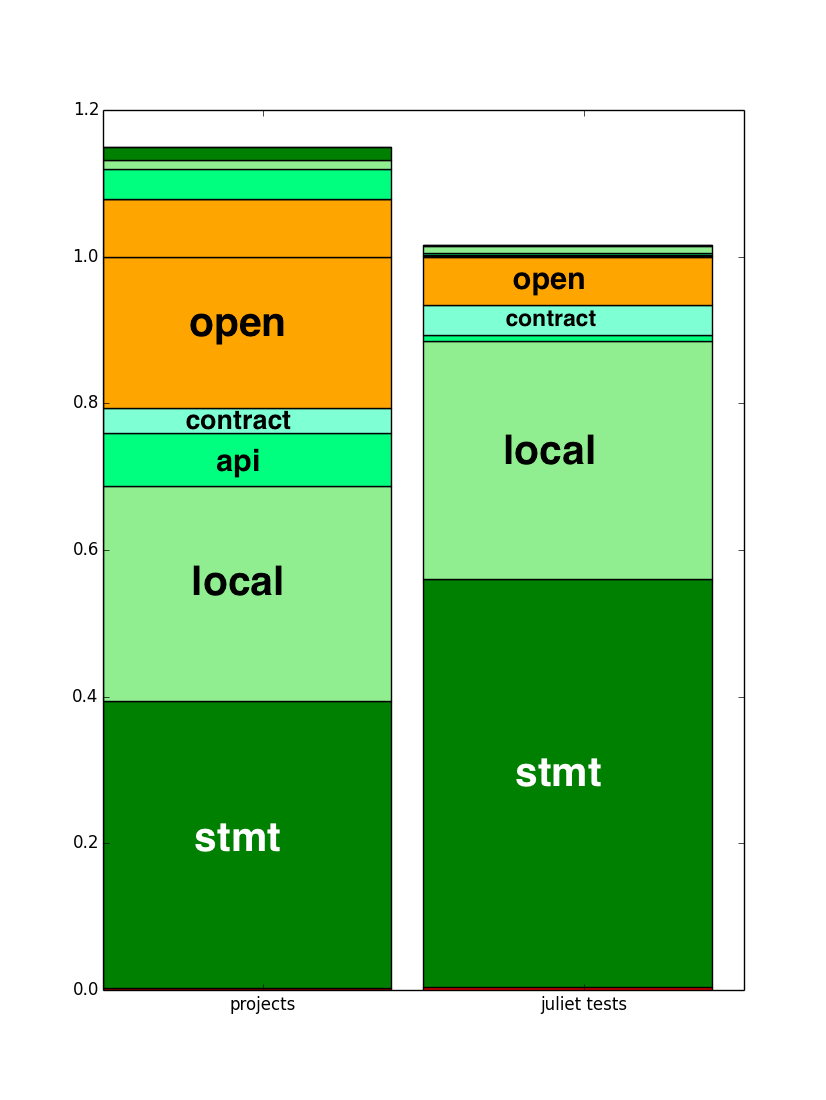
\includegraphics[width=.6\textwidth]{projects_vs_juliet.png}
\end{center}
\caption{\label{fig:appvsjuliet}Comparison in proof obligation discharge methods between
applications and the Juliet test suites}
\end{figure}

We have applied KT Advance to several real-world applications, with a total of over
1.5 million lines of code across several application domains. Applications include
openssl,  lighttpd (server), nagios (enterprise), cairo (graphics), 
wpa\_supplicant (wifi), dovecot (email),  nginx. Figure~\ref{fig:appvsjuliet} shows
a comparison of the relative fractions and methods of proof obligation discharge for
these applications and for the juliet tests. The figure shows the percentages of
proof obligations that were discharged (or not) using one of the following methods:
\begin{itemize}
\item {\bf stmt} The proof obligation is proven safe based exclusively on information
present in the statement itself or in its associated declarations; to discharge proof
obligations requires very little analysis capability beyond what a regular compiler
may already provide.
\item {\bf local} The proof obligation is proven safe based exclusively on information
present in the function itself; to discharge proof obligations requires data flow
analysis capabilities in different domains to propagate values and relationships. 
Context-sensitive analysis is not required to discharge these proof obligations.
\item {\bf api} The proof obligation can only be proven safe by making assumptions
on the arguments passed to the function (e.g., requiring that a pointer argument is
not-null, or that an integer value is non-negative), which in turn requires that 
these assumptions be satisfied by the callers of this function. These proof obligations
thus require context-sensitive analysis capabilities.
\item {\bf contract} The proof obligation needs additional information and assumptions
beyond the information provided in the first three categories, which may include 
assumptions about global variables, external assumptions (e.g., that {\tt stdin} is
not null) or function post condition guarantees. 
\item {\bf open} KT Advance, at the time of writing of this report, is not able to
discharge these proof obligations.
\end{itemize}
The figure shows both the \emph{primary proof obligations}, which are the conditions that
are  automatically generated for all constructs that can lead to undefined behavior
(or some other undesirable state) and the \emph{supporting proof obligations} (above 1.0)
with the same color coding.

Comparing the two bar graphs we observe the following:
\begin{itemize}
\item  The fraction of ``easy'' proof obligations in the Juliet Test Suite is close to 60\%,
while in real-world code this is just 40\%, indicating that the Juliet Test Suite code
is considerably simpler in terms of constructs used.
\item The fraction of {\tt api}-delegated proof obligations in the Juliet Test Suite is less
than 1\%, while in the real-world code the {\tt api}-delegated proof obligations make up
more than 6\%, indicating that real-world code requires significantly more context-sensitive
reasoning capability to judge proof obligations.
\item The fraction of {\tt contract}-delegated proof obligations in the Juliet Test Suite
is slightly higher than that for real-world code. This is attributable to the fact that the use of global
variables in the Juliet Test Suite is rather uniform and easy to capture in contract 
conditions, and enables automatic 
generation of contracts, which is generally not the case for real-world code.
\item The number of supporting proof obligations (expressed as a relative fraction of the
number of primary proof obligations) is much smaller for the Juliet Test Suite than for 
real-world code, again indicating the very limited context-sensitivity required for the
Juliet Test Suite, compared to real-world code.
\end{itemize}

\begin{figure}[h]
\begin{center}
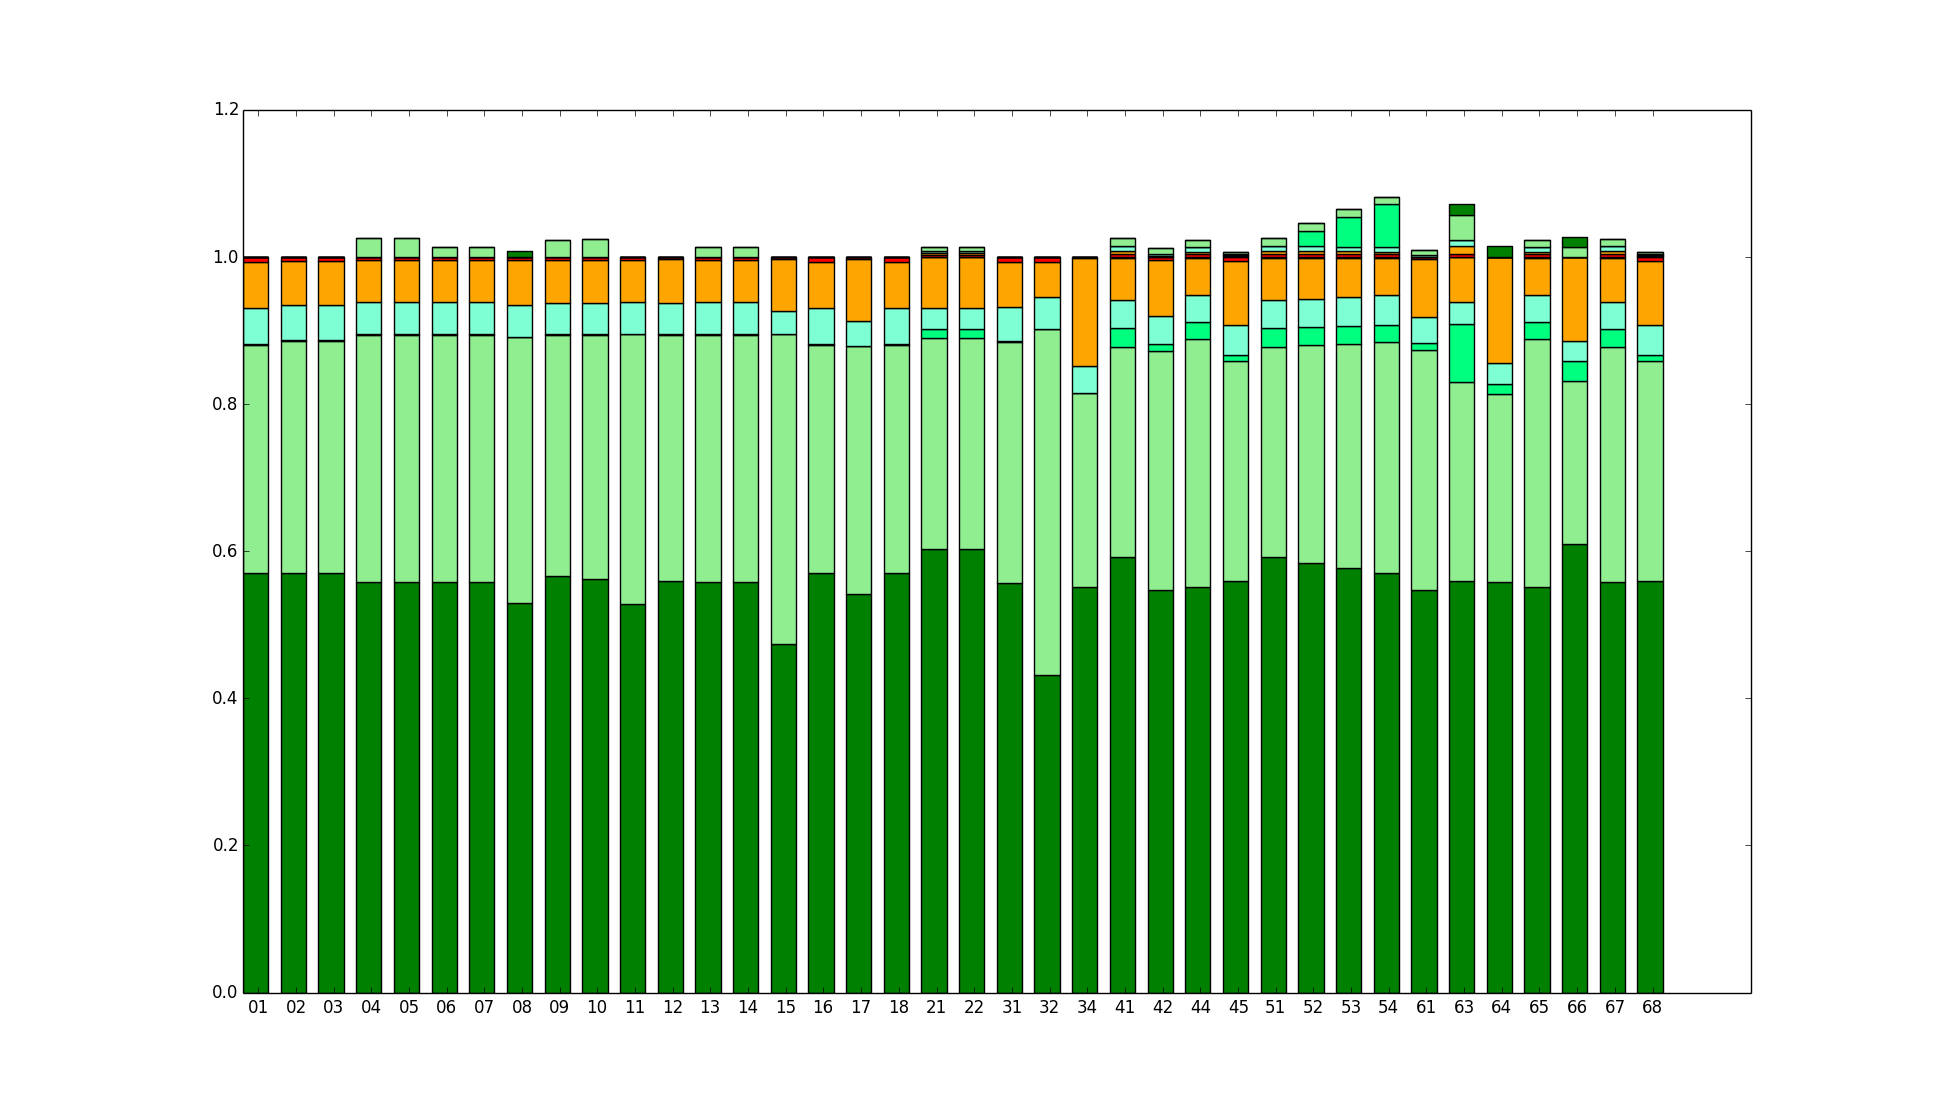
\includegraphics[width=\textwidth]{juliet_variants_fractions.png}
\end{center}
\caption{\label{fig:julietvariants}Proof obligation discharge methods for the different
control/data flow variants of the juliet tests}
\end{figure}

\begin{figure}[h]
\begin{center}
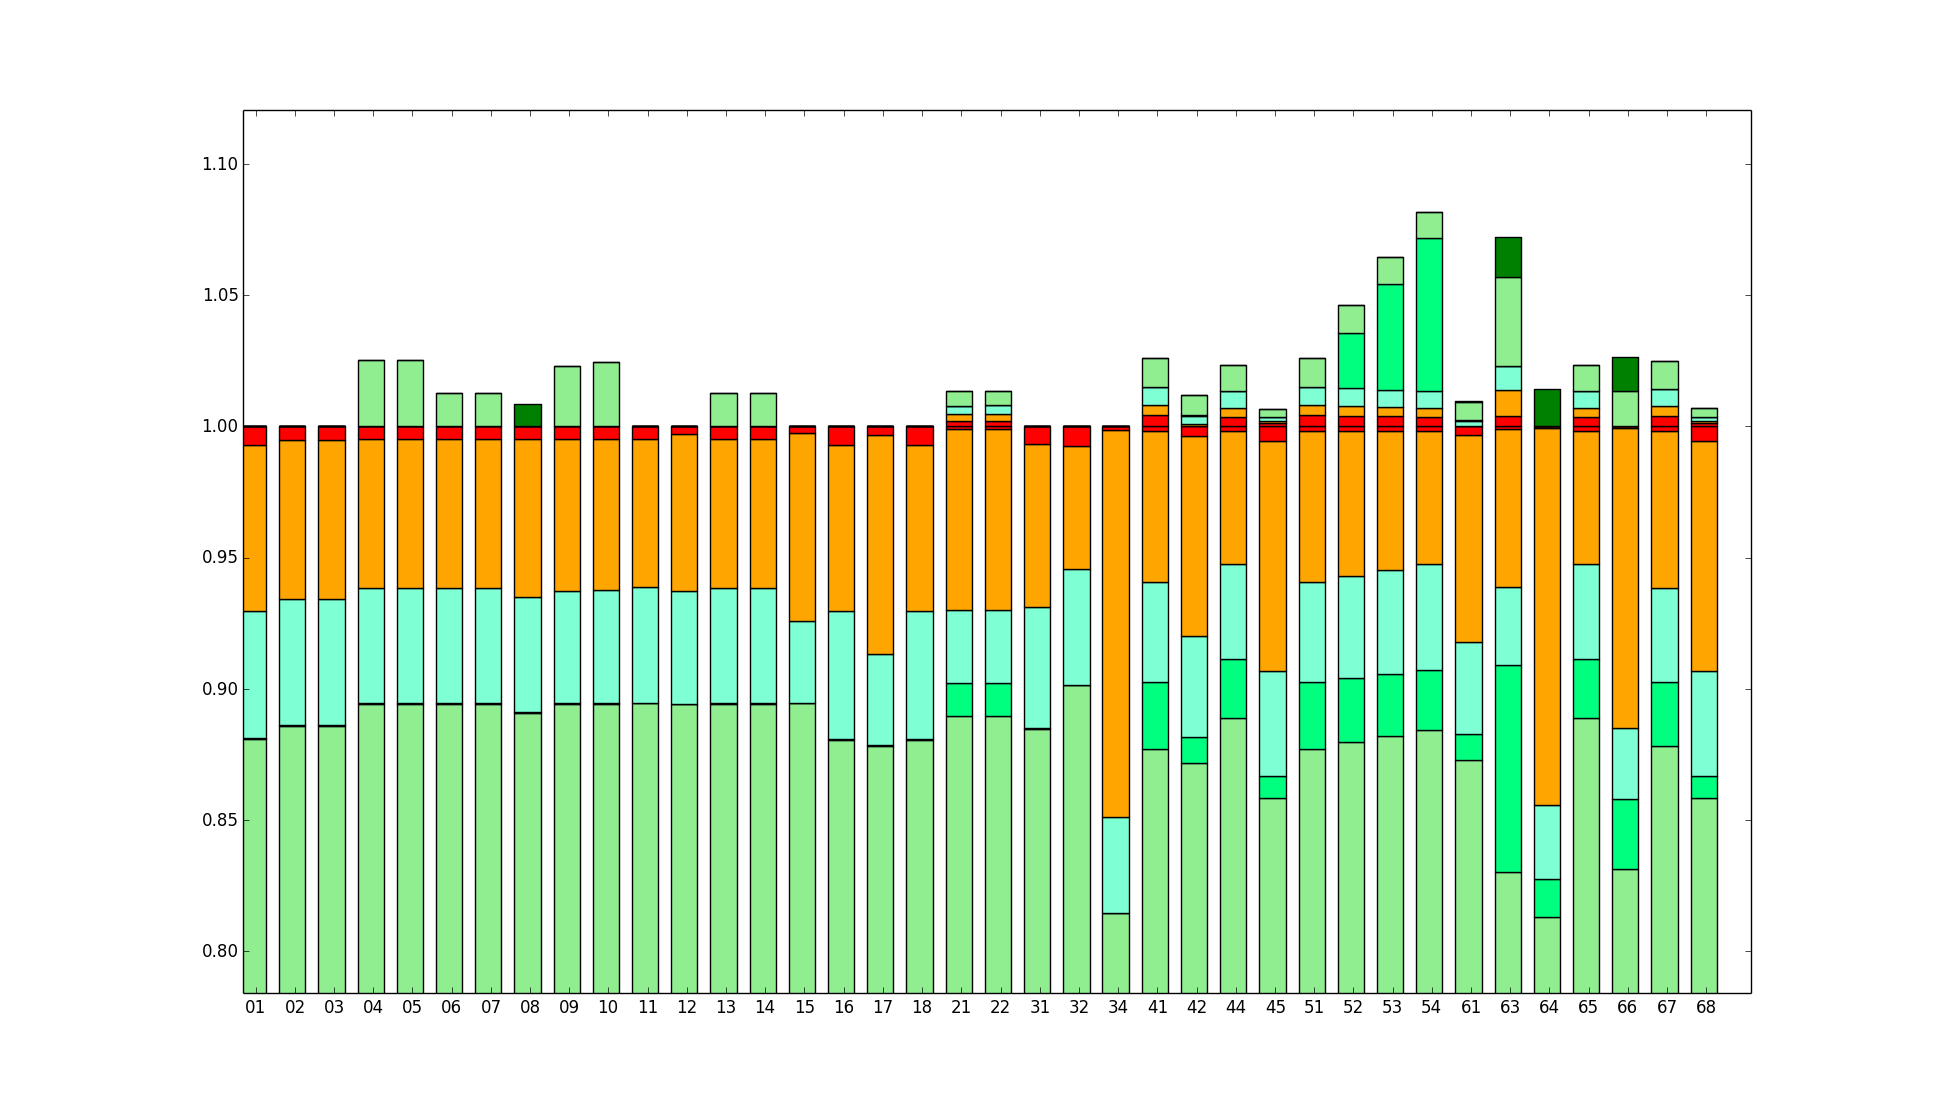
\includegraphics[width=\textwidth]{juliet_variants_fractions_zoom.png}
\end{center}
\caption{\label{fig:julietvariantszoom}Proof obligation discharge methods for the different
control/data flow variants  of the juliet tests (enlarged)}
\end{figure}


The Juliet Test Suite evaluates the capability of analysis tools for different control
flow and data flow constructs by providing 18, 34, or 38 flow variants for each 
functional variant.
Figures~\ref{fig:julietvariants} show the analysis results for the combined 38 flow variants;
a partial view of the top part of the bars is shown in Figure~\ref{fig:julietvariantszoom}.
The figures show that indeed there is some variability in analysis difficulty (or 
need for more advanced analysis capabilities) for different flow variants. Clearly
flow variants 51-54 require increasing levels of context sensitive analysis (judging
from the increasing numbers of supporting proof obligations). 
Flow variants 34 (use of unions) and 64 (use of void pointers to pass data are around)
are more difficult to analyze, at least for KT Advance (leaving more proof obligations
open). Overall, however, the variability in analysis difficulty between the different
flow variants is limited, especially if we compare these results with the analogous
results for real-world code.

\begin{figure}[h]
\begin{center}
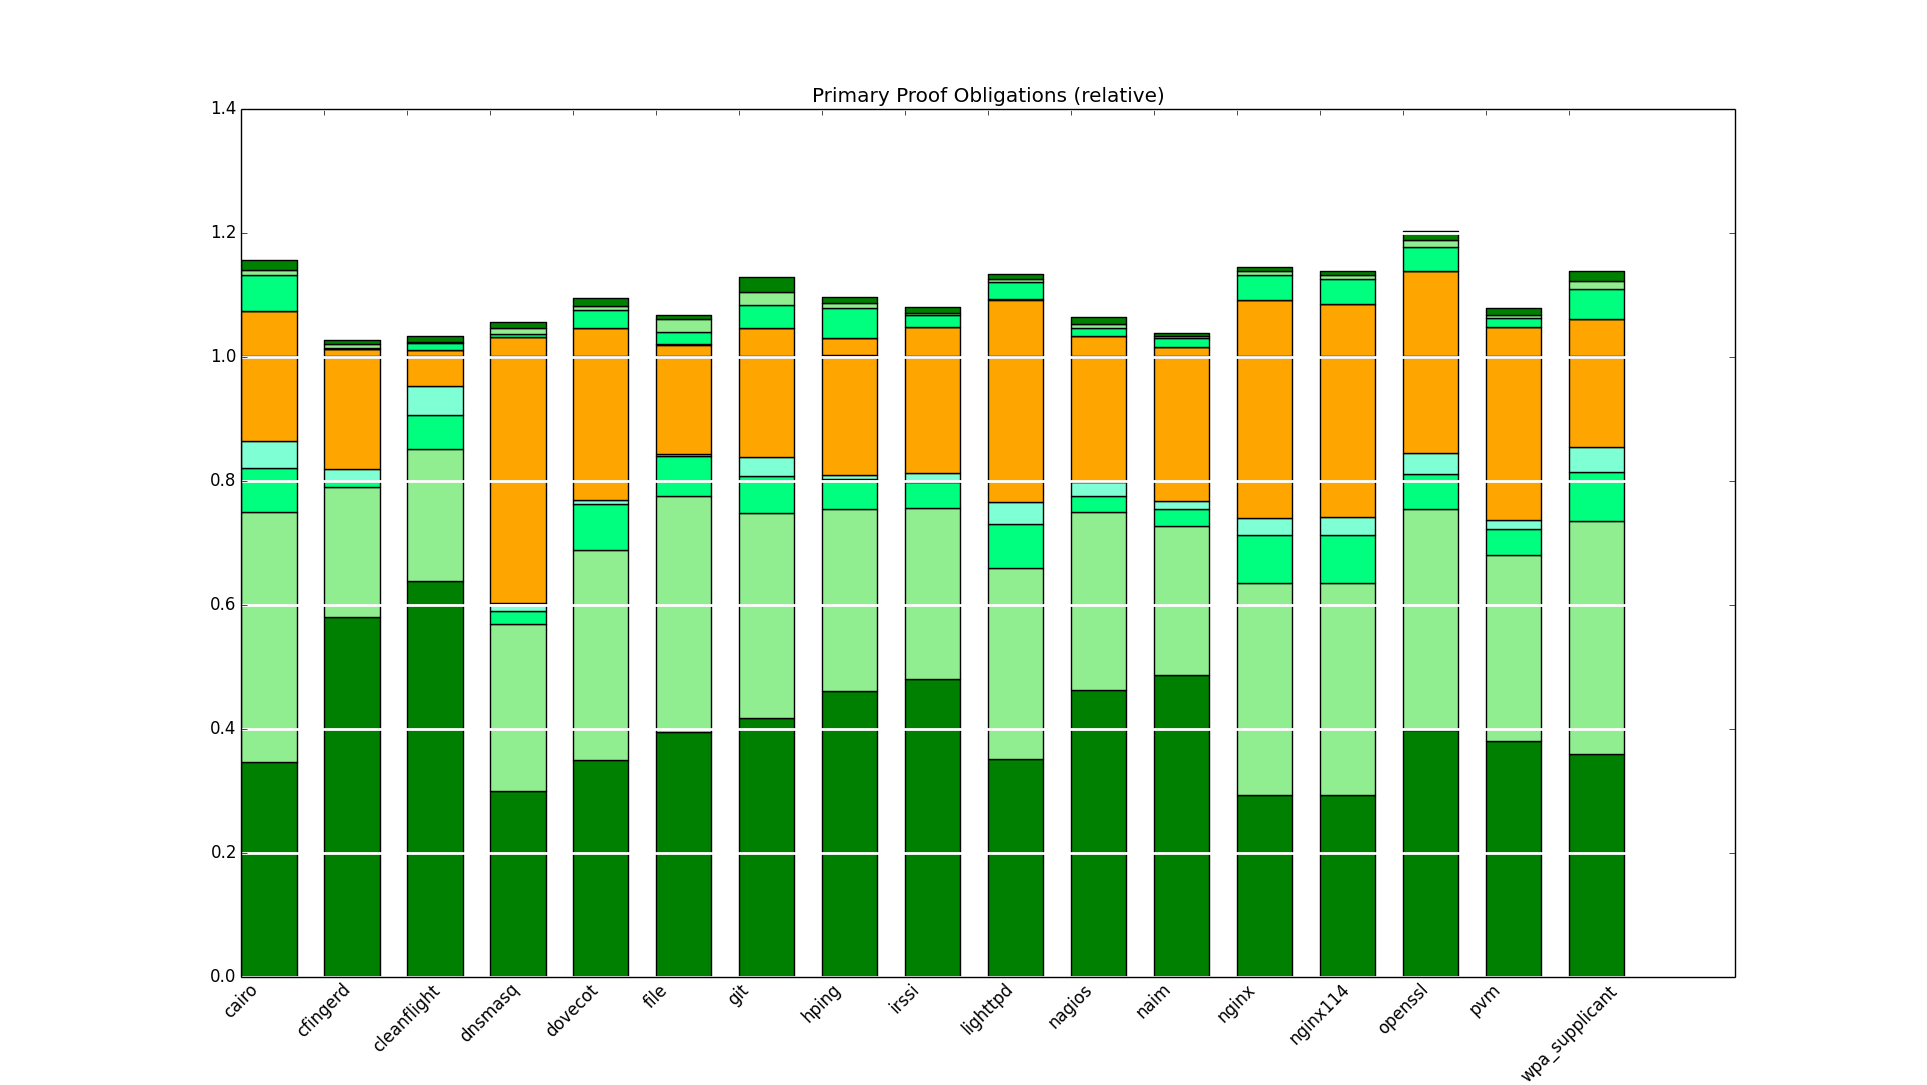
\includegraphics[width=\textwidth]{projects_fractions.png}
\end{center}
\caption{\label{fig:appstats}Proof obligation discharge methods for several real-world applications}
\end{figure}

Figure~\ref{fig:appstats} shows the relative distribution of proof obligation discharge
methods for a set of real-world applications that we have analyzed with KT Advance. The
figure shows that there is a large variability in ``ease of analysis'' for the different
applications, with {\tt cleanflight}, an embedded system, being similar to the Juliet Test
Suite in its distribution and {\tt dnsmasq} and the {\tt nginx} versions exhibiting a much
lower level of ``simple'' proof obligation discharges. Clearly performance on the Juliet
Test Suite is not representative of how a static analysis tool might perform  on these 
applications. Also the number of supporting proof obligations is much higher, reaching
almost 20\% of the number of primary proof obligations for {\tt openssl}, tends to be
much higher for real-world applications, indicating much longer call chains and, in
general, more inter-procedural dependencies than present in the Juliet Test Suite tests.

\begin{figure}[h]
\begin{center}
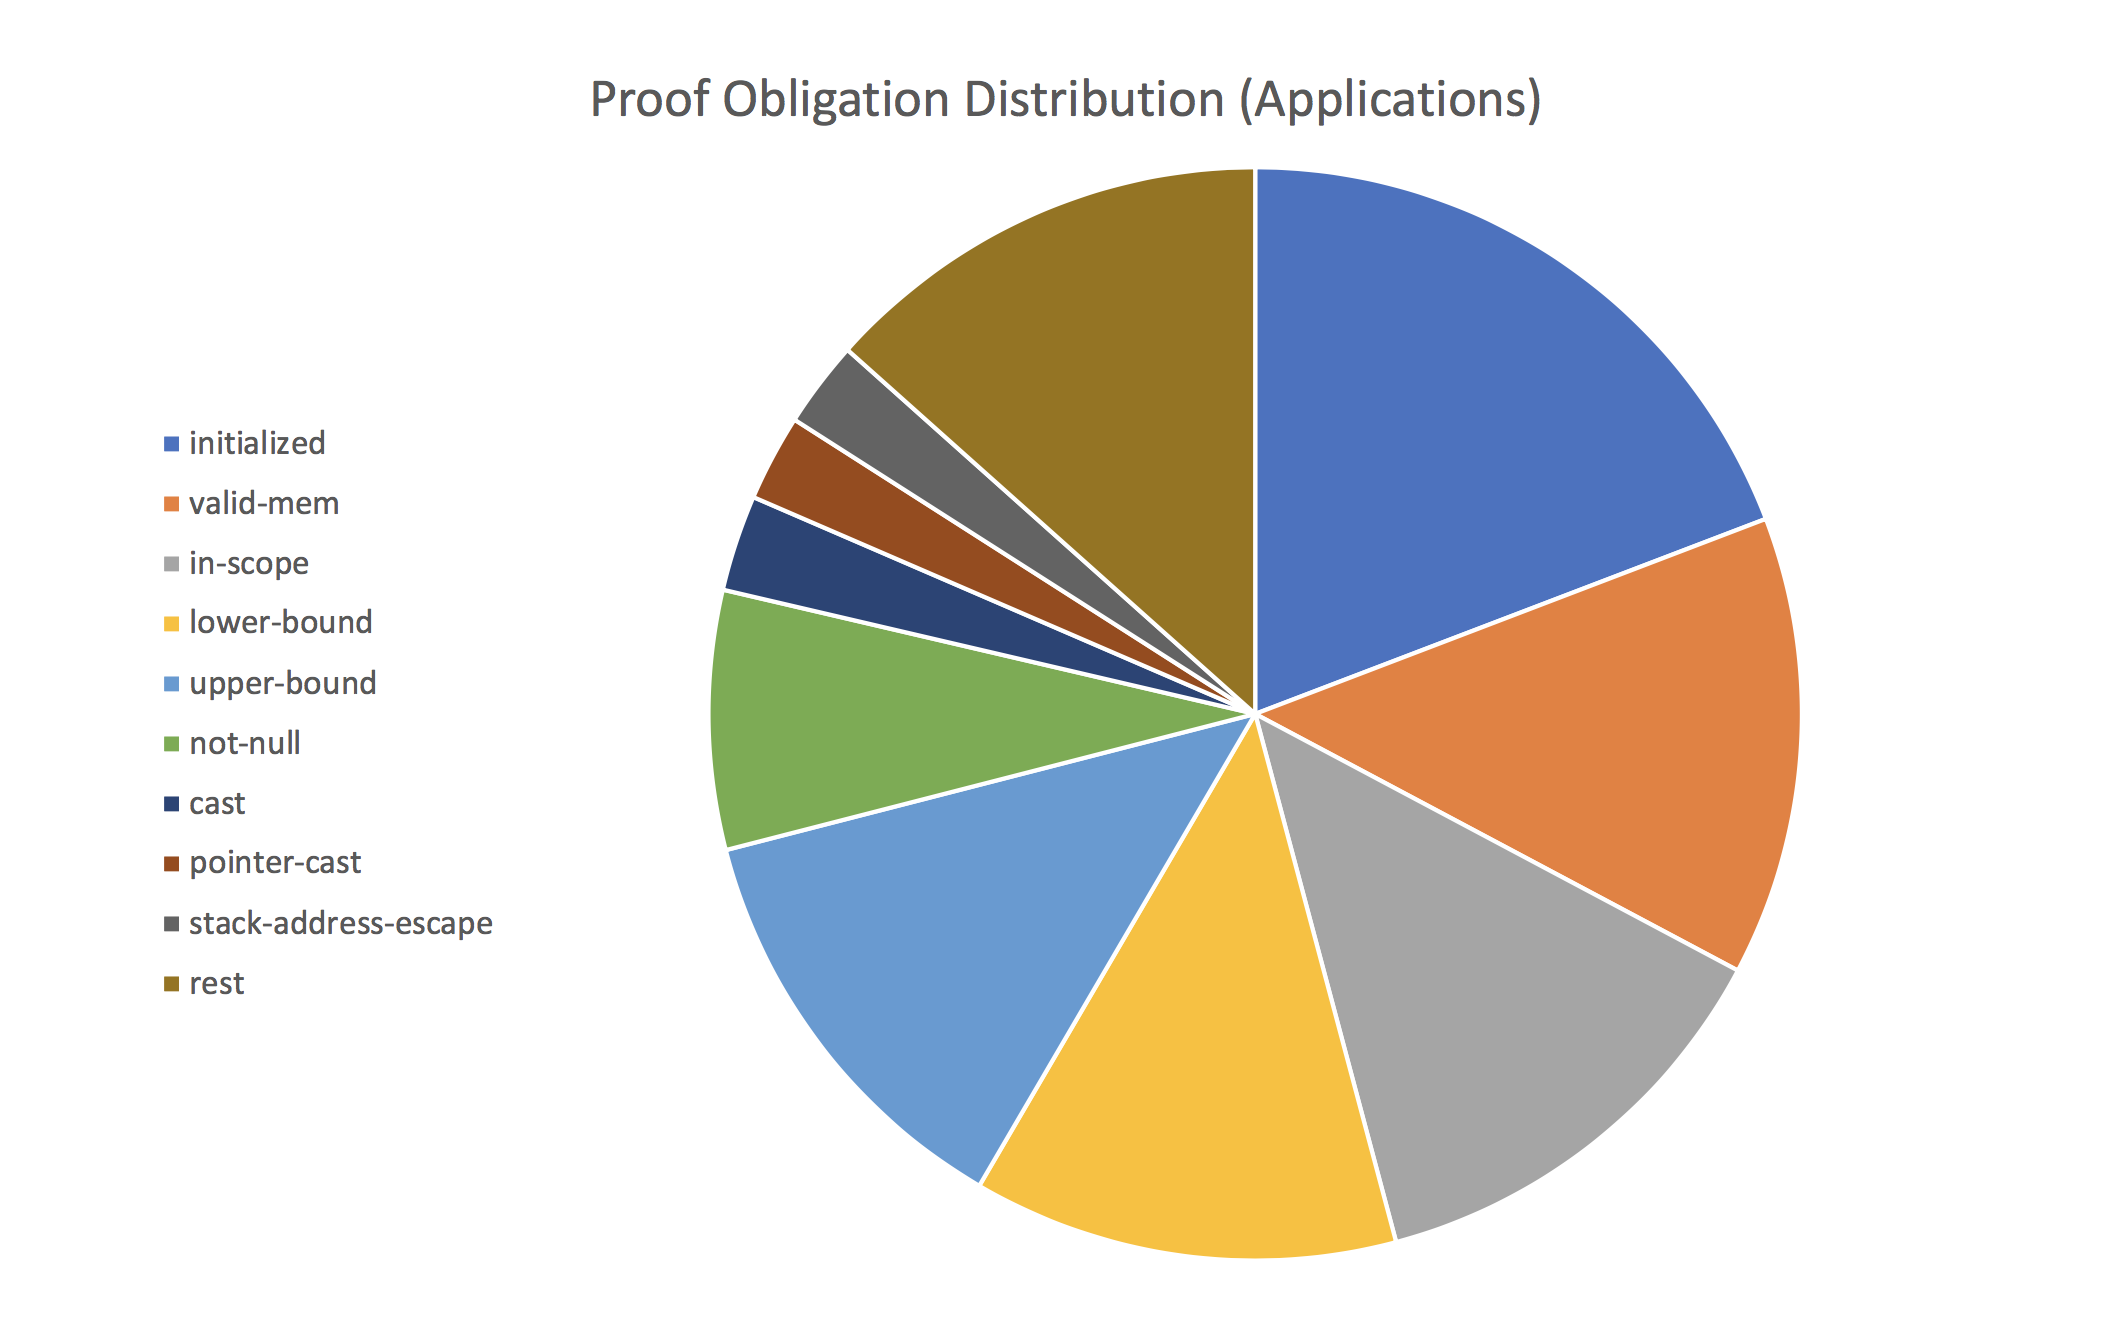
\includegraphics[width=.8\textwidth]{pie_apps.png}
\end{center}
\caption{\label{fig:pie}Proof obligation distribution for several real-world applications}
\end{figure}

\begin{figure}[h]
\begin{center}
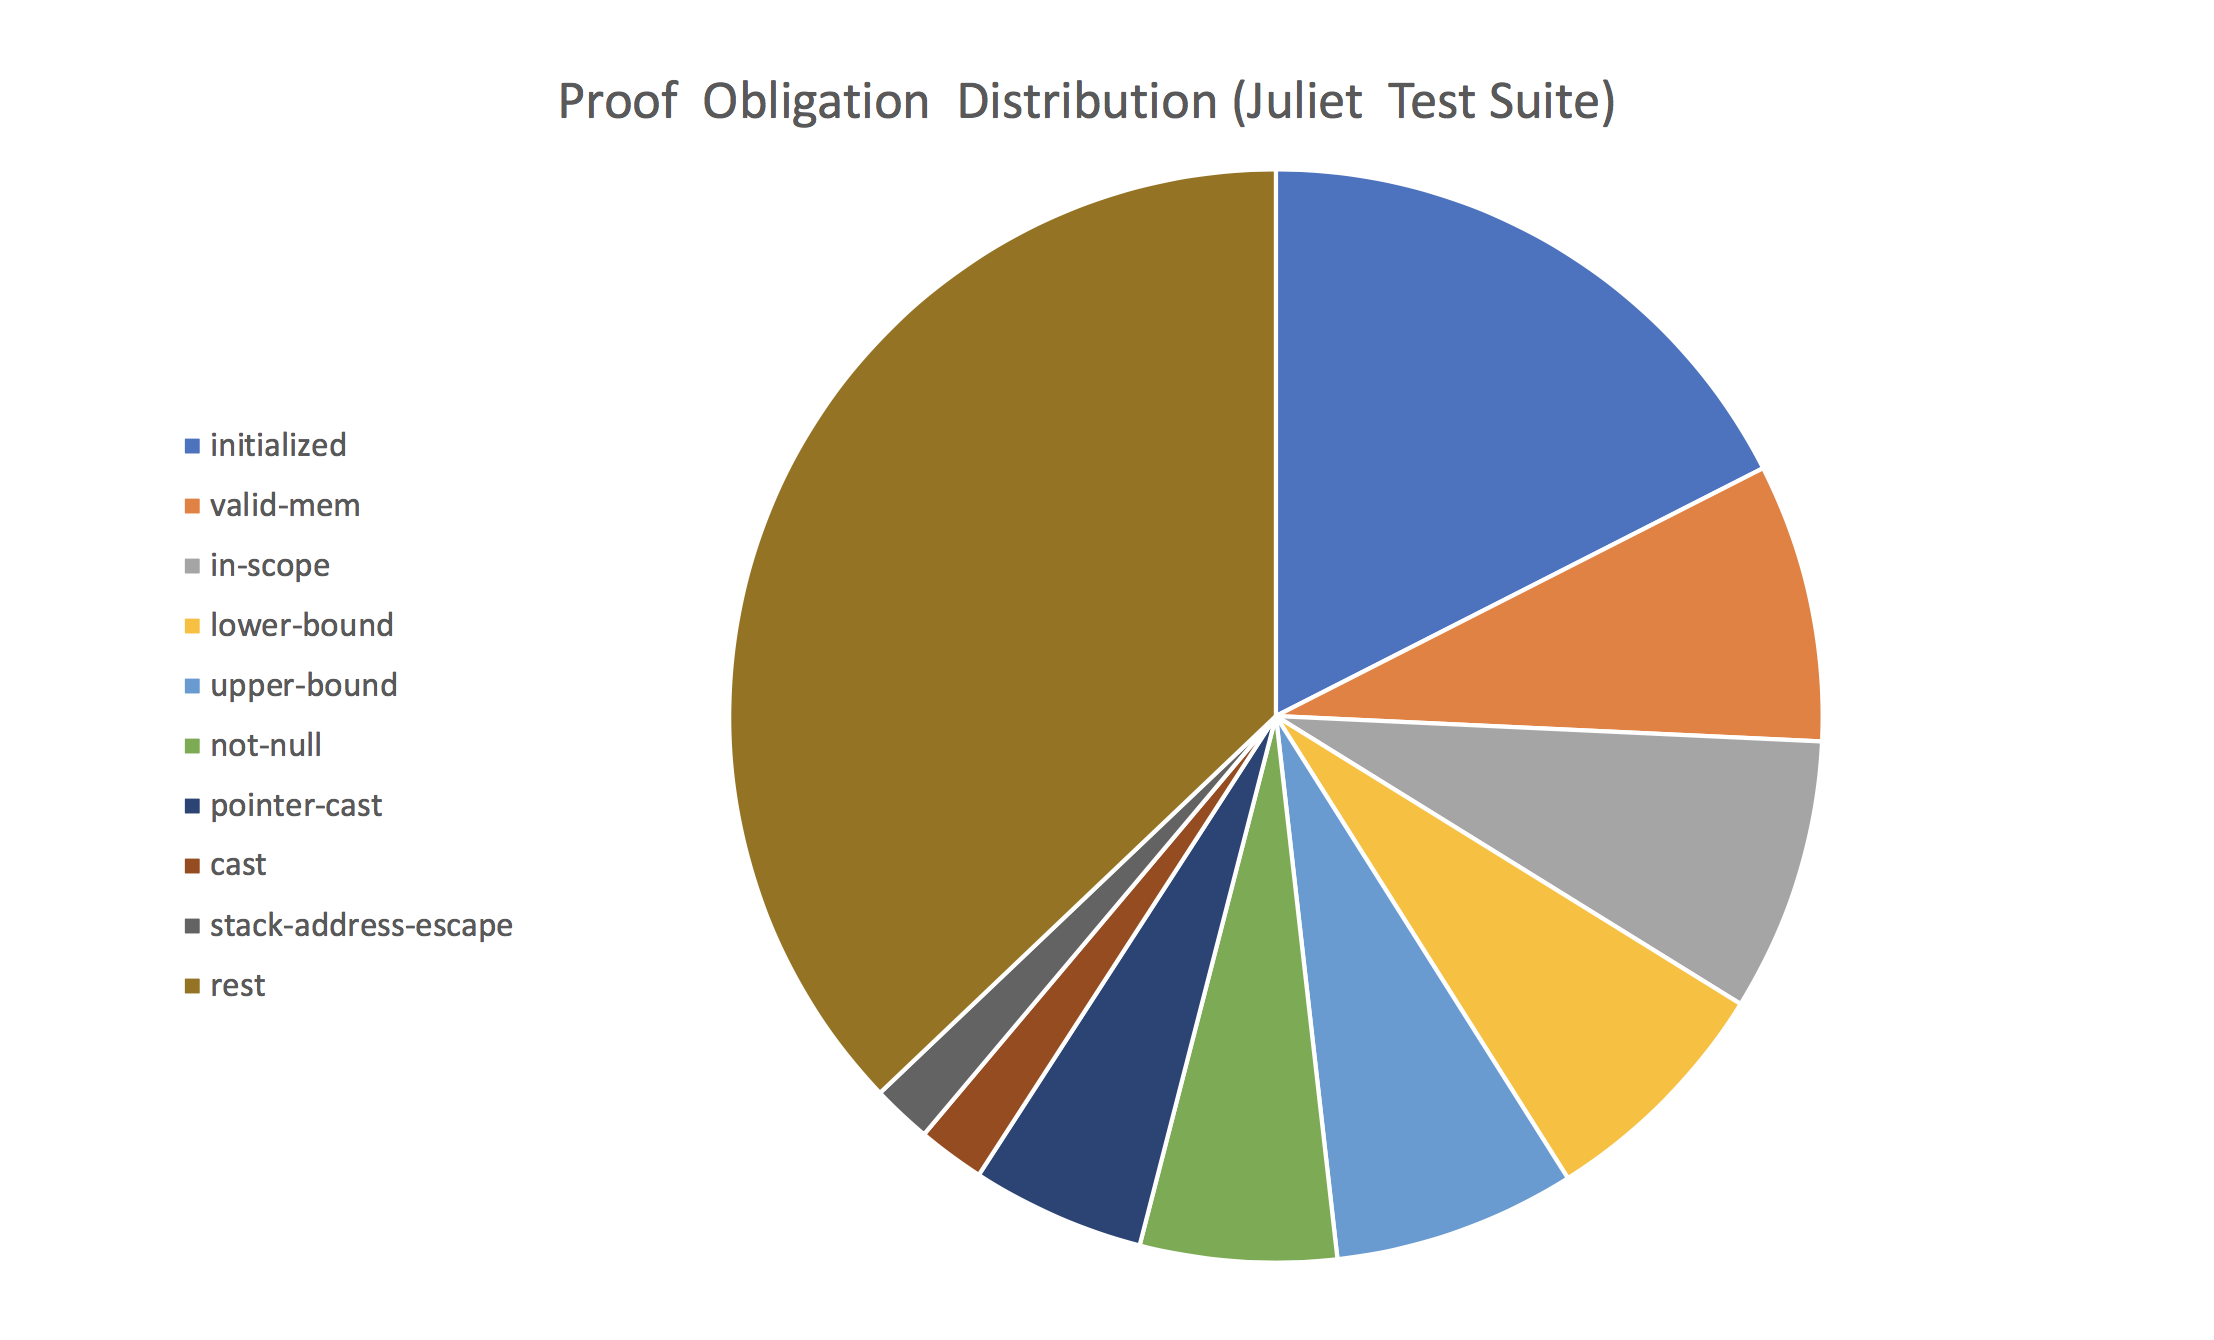
\includegraphics[width=.8\textwidth]{pie_juliet1.png}
\end{center}
\caption{\label{fig:jpie1}Proof obligation distribution for Juliet Test Suite}
\end{figure}

\begin{figure}[h]
\begin{center}
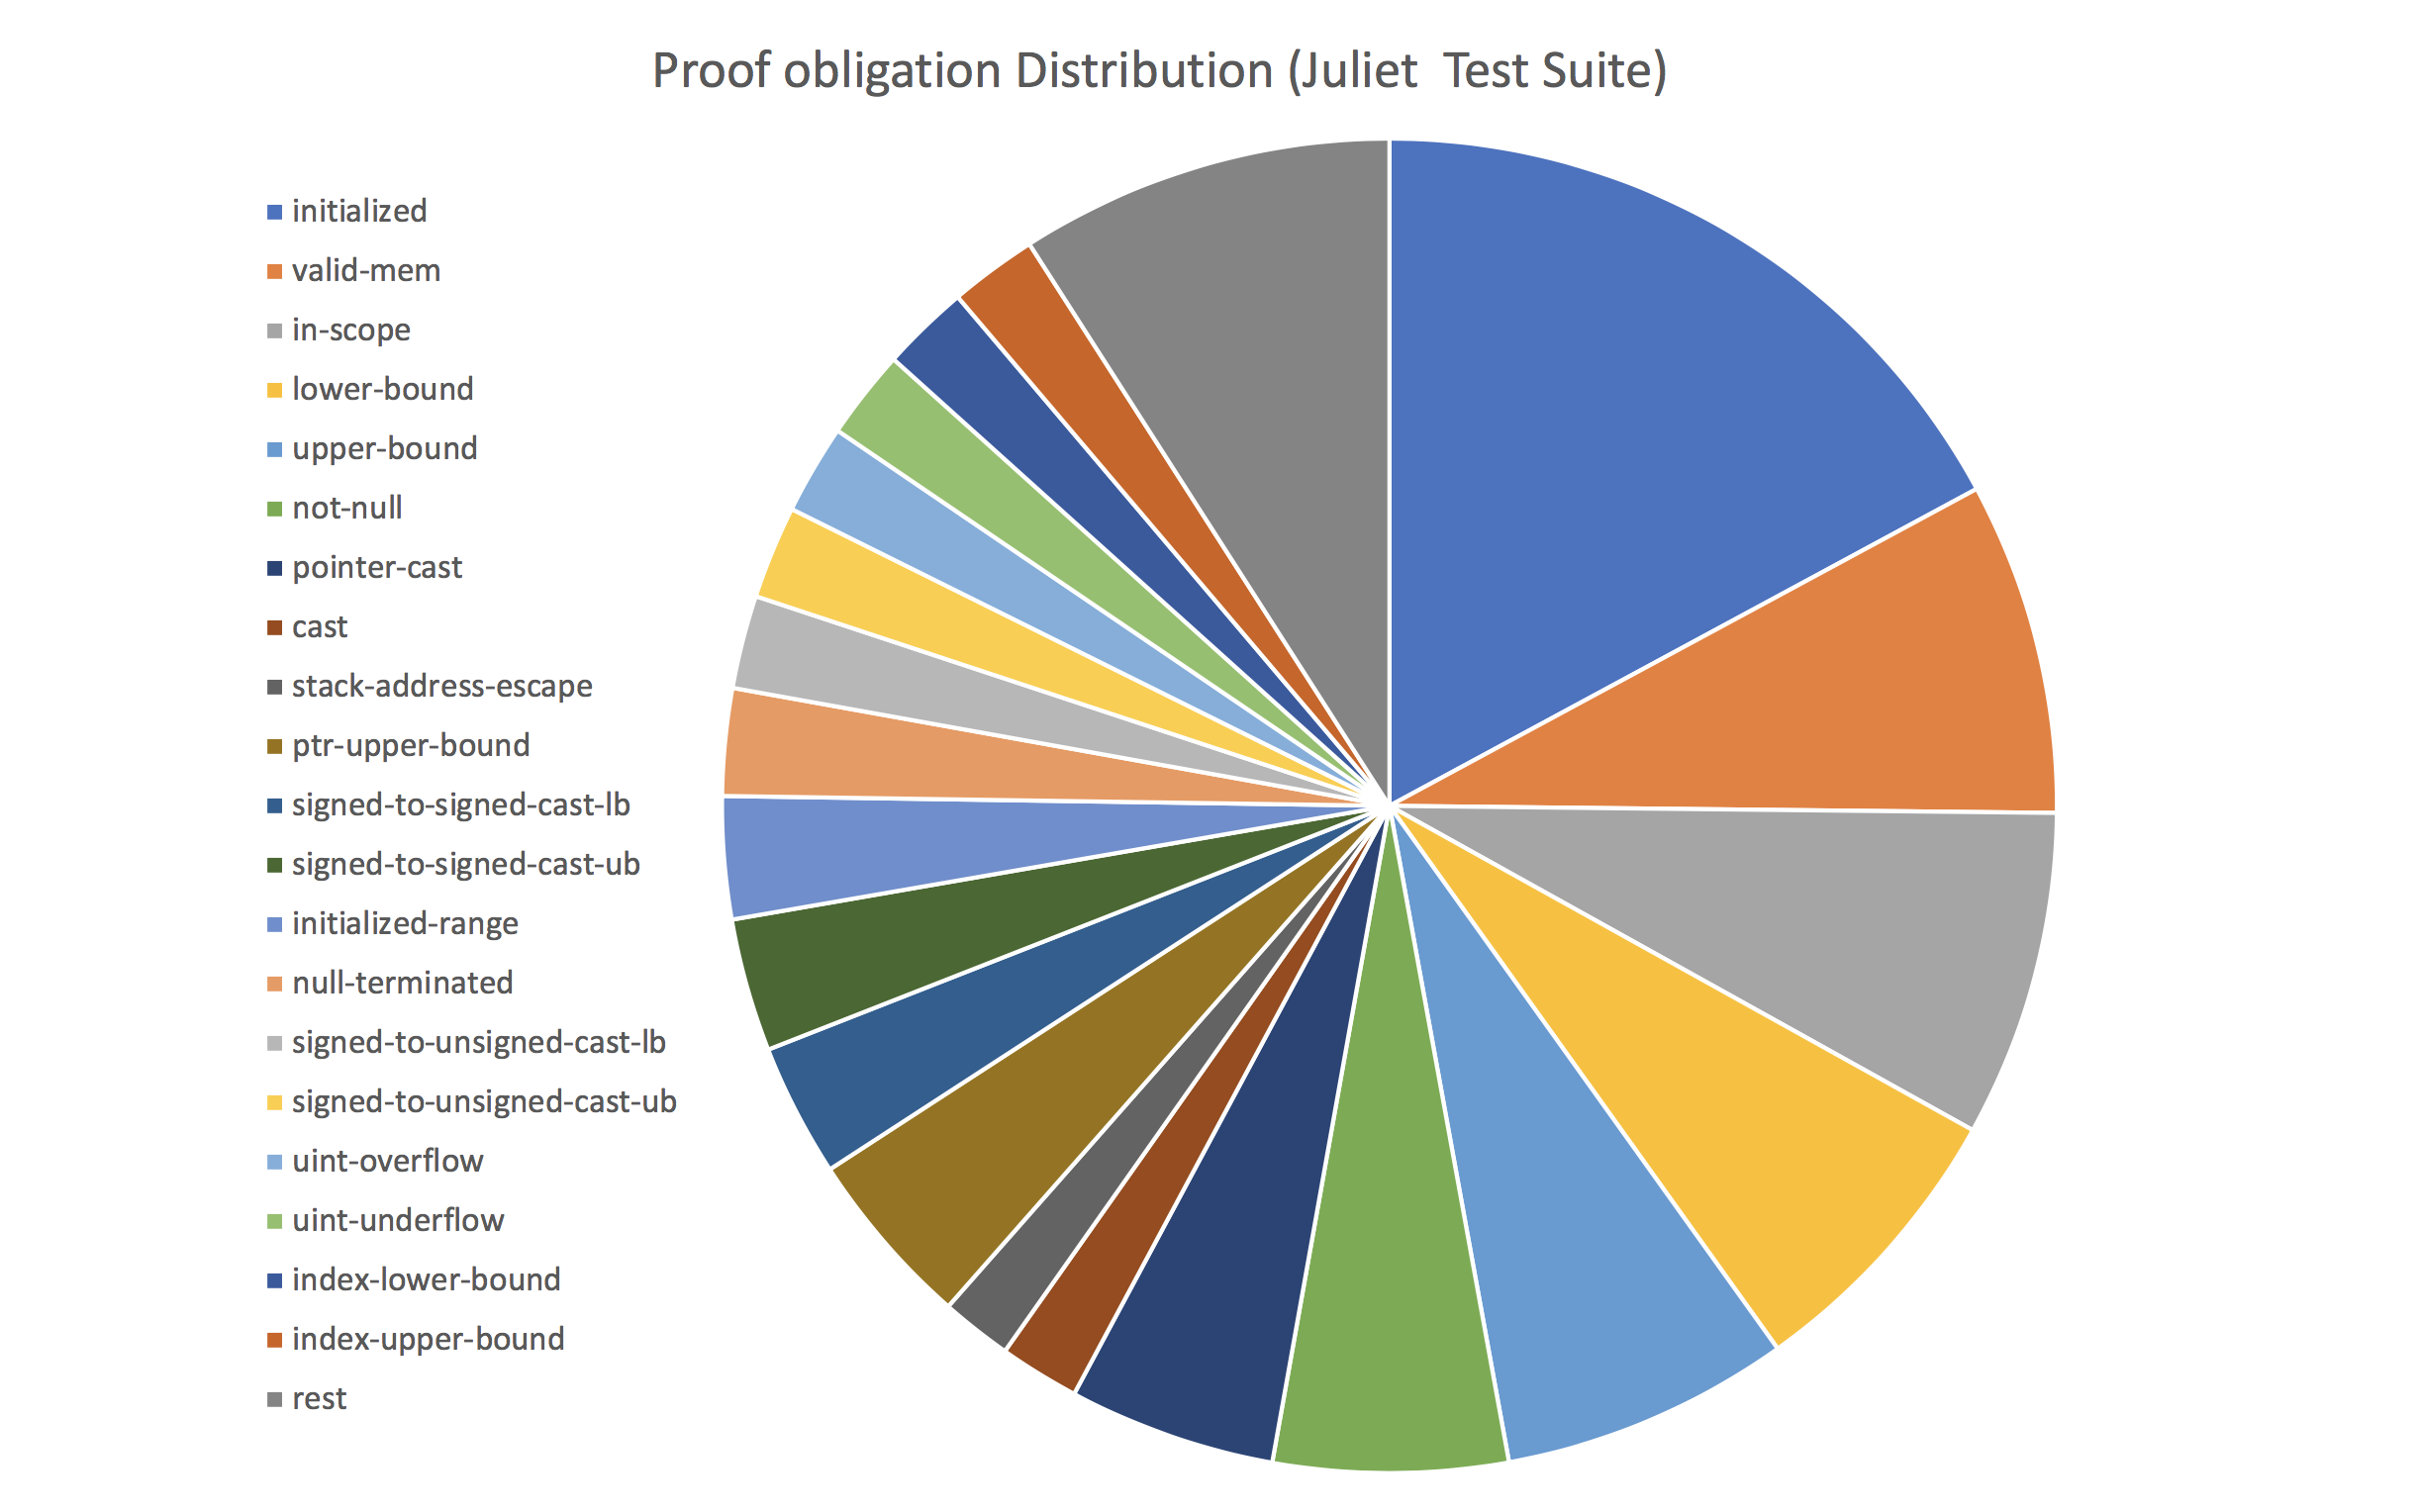
\includegraphics[width=.8\textwidth]{pie_juliet2.png}
\end{center}
\caption{\label{fig:jpie2}Proof obligation distribution for Juliet Test Suite}
\end{figure}

Another difference between the Juliet Test Suite and the real-world applications is the
distribution of proof obligation predicates. Figure~\ref{fig:pie} shows that for the
real world applications  the nine
most common proof obligation predicates make up about 80\% of all proof obligations.
For the Juliet Test Suite Figure~\ref{fig:jpie1} shows that these same nine proof 
obligation predicates make up only about 60\% of all proof obligations. Figure~\ref{fig:jpie2}
shows the contribution of several other proof obligations whose individual percentages
exceed  3\%. Especially the contribution of the predicates {\tt initialized-range}
and {\tt null-terminated} is much higher than in real-world code, reflecting the many
strings being used in these tests. Also the contribution of the predicates
{\tt index-lower-bound} and {\tt index-upper-bound} (for declared arrays) is much
larger than in real code, where most operations involve pointers rather than arrays,
explaining perhaps some of the difference in analysis difficulty as array bound
checking is much easier than pointer bounds checking, as arrays carry their size
(upper bound) with them, while this upper bound must be separately derived for
pointers into buffers.


\section{Conclusions and Recommendations}
\label{sec:recs}

The Juliet Test Suite is a great asset for tool developers: it systematically exercises
many of the possible violations in many different contexts, allowing tool developers to
perform extensive testing and evaluation of their tools to uncover any corner cases 
that may not be handled correctly. It is less clear, however, whether the test suite
is as useful as an evaluation tool
to assess the capabilities of static analysis tools on real code due to the much more
limited scope of code constructs and code complexity exhibited by the tests. 

As indicated in both ~\cite{Juliet12} and \cite{NIST1995} the best test suite for
evaluation is actual production code with all issues labeled. We are currently working
on the creation of a reference verification of the applications mentioned above, which
range from 5000 to 400,000 lines of code. We recommend more support for this approach
as it would achieve two desirable goals at once: improve the capabilities of sound
static analysis and produce realistic test suites. 



\bibliography{citations}
\bibliographystyle{acm}

\newpage

\appendix

\section{Juliet Test Cases Covered}
\label{app:tests}

Table~\ref{tab:cwes} lists the CWEs with the number of tests in that CWE
that have been analyzed by KT Advance so far and that have been included
in this study.

\begin{table}[h]
\begin{tabular}{c|l|r}
CWE & description & tests \\ \hline
121 & stack-based buffer overflow &  1894  \\
122 & heap-based buffer overflow  &  1670 \\
123 & write-what-where condition & 114 \\
124 & buffer underwrite & 720 \\
126 & buffer overread  & 562 \\
127 & buffer underread &  720 \\
134 & uncontrolled format string & 950 \\
188 & reliance on data memory layout & 36 \\
190 & integer overflow & 3420 \\
191 & integer underflow & 2622 \\
194 & unexpected sign extension & 342 \\
195 & signed-to-unsigned conversion error & 646 \\
196 & unsigned-to-signed conversion error & 18 \\
197 & numeric truncation error & 38 \\
242 & use of inherently dangerous function & 18 \\
252 & unchecked return value & 18 \\
253 & incorrect check of function return value & 126 \\
369 & division by zero & 684 \\
391 & unchecked error condition & 18 \\
415 & double free & 38 \\
416 & use after free & 118 \\
457 & use of uninitialized variable & 80 \\
469 & use of pointer subtraction to determine size & 18 \\
476 & null pointer dereference & 53 \\
562 & return of stack variable address & 2 \\
587 & assignment of fixed address to pointer & 18 \\
588 & attempt to access child of non-structure pointer & 34 \\
590 & free memory not on heap &  306 \\
665 & improper initialization & 76 \\
680 & integer overflow to buffer overflow & 152 \\
681 & incorrect conversion between numeric types & 54 \\
685 & function call with incorrect number of arguments & 18 \\
688 & function call with incorrect variable or reference as argument & 18 \\
758 & undefined behavior & 90 \\
761 & free pointer not at start of buffer & 152 \\ \hline
 & & 15,843
\end{tabular}
\caption{\label{tab:cwes} Tests included in our study}
\end{table}

\section{Scorekey Example}
\label{app:scorekey}
\begin{tiny}
\begin{verbatim}
{
    "test": "CWE121/s01/CWE129_large",
    "macros": {
        "PPO1": {
            "P": "index-upper-bound"
        },
        "PS1": [ "PPO1" ]
    },
    "tests": {
        "01": {
            "cfiles": {
                "x01.c": {
                    "violations": {
                        "36": [ "PS1" ]
                    },
                    "safe-controls": {
                        "70": [ "PS1" ],
                        "98": [ "PS1" ]
                    }
                }
            }
        },
        "02": {
            "cfiles": {
                "x02.c": {
                    "violations": {
                        "41": [ "PS1" ]
                    },
                    "safe-controls": {
                        "84": [ "PS1" ],
                        "118": [ "PS1" ],
                        "159": [ "PS1" ]
                    }
                }
            }
        },
        "03": {
            "cfiles": {
                "x03.c": {
                    "violations": {
                        "41": [ "PS1" ]
                    },
                    "safe-controls": {
                        "84": [ "PS1" ],
                        "118": [ "PS1" ],
                        "159": [ "PS1" ]
                    }
                }
            }
        },
        "04": {
            "cfiles": {
                "x04.c": {
                    "violations": {
                        "47": [ "PS1" ]
                    },
                    "safe-controls": {
                        "90": [ "PS1" ],
                        "124": [ "PS1" ],
                        "165": [ "PS1" ],
                        "201": [ "PS1" ]
                    }
                }
            }
        },
        "05": {
            "cfiles": {
                "x05.c": {
                    "violations": {
                        "47": [ "PS1" ]
                    },
                    "safe-controls": {
                        "90": [ "PS1" ],
                        "124": [ "PS1" ],
                        "165": [ "PS1" ],
                        "201": [ "PS1" ]
                    }
                }
            }
        },
        "06": {
            "cfiles": {
                "x06.c": {
                    "violations": {
                        "46": [ "PS1" ]
                    },
                    "safe-controls": {
                        "89": [ "PS1" ],
                        "123": [ "PS1" ],
                        "164": [ "PS1" ],
                        "200": [ "PS1" ]
                    }
                }
            }
        },
        "07": {
            "cfiles": {
                "x07.c": {
                    "violations": {
                        "46": [ "PS1" ]
                    },
                    "safe-controls": {
                        "89": [ "PS1" ],
                        "123": [ "PS1" ],
                        "164": [ "PS1" ],
                        "200": [ "PS1" ]
                    }
                }
            }
        },
        "08": {
            "cfiles": {
                "x08.c": {
                    "violations": {
                        "54": [ "PS1" ]
                    },
                    "safe-controls": {
                        "97": [ "PS1" ],
                        "131": [ "PS1" ],
                        "172": [ "PS1" ],
                        "208": [ "PS1" ]
                    }
                }
            }
        },
        "09": {
            "cfiles": {
                "x09.c": {
                    "violations": {
                        "41": [ "PS1" ]
                    },
                    "safe-controls": {
                        "84": [ "PS1" ],
                        "118": [ "PS1" ],
                        "159": [ "PS1" ],
                        "195": [ "PS1" ]
                    }
                }
            }
        },
        "10": {
            "cfiles": {
                "x10.c": {
                    "violations": {
                        "41": [ "PS1" ]
                    },
                    "safe-controls": {
                        "84": [ "PS1" ],
                        "118": [ "PS1" ],
                        "159": [ "PS1" ],
                        "195": [ "PS1" ]
                    }
                }
            }
        },
        "11": {
            "cfiles": {
                "x11.c": {
                    "violations": {
                        "41": [ "PS1" ]
                    },
                    "safe-controls": {
                        "84": [ "PS1" ],
                        "118": [ "PS1" ],
                        "159": [ "PS1" ],
                        "195": [ "PS1" ]
                    }
                }
            }
        },
        "12": {
            "cfiles": {
                "x12.c": {
                    "violations": {
                        "47": [ "PS1" ]
                    },
                    "safe-controls": {
                        "68": [ "PS1" ],
                        "113": [ "PS1" ],
                        "134": [ "PS1" ],
                        "178": [ "PS1" ],
                        "200": [ "PS1" ]
                    }
                }
            }
        },
        "13": {
            "cfiles": {
                "x13.c": {
                    "violations": {
                        "41": [ "PS1" ]
                    },
                    "safe-controls": {
                        "84": [ "PS1" ],
                        "118": [ "PS1" ],
                        "159": [ "PS1" ],
                        "195": [ "PS1" ]
                    }
                }
            }
        },
        "14": {
            "cfiles": {
                "x14.c": {
                    "violations": {
                        "41": [ "PS1" ]
                    },
                    "safe-controls": {
                        "84": [ "PS1" ],
                        "118": [ "PS1" ],
                        "159": [ "PS1" ],
                        "195": [ "PS1" ]
                    }
                }
            }
        },
        "15": {
            "cfiles": {
                "x15.c": {
                    "violations": {
                        "48": [ "PS1" ]
                    },
                    "safe-controls": {
                        "102": [ "PS1" ],
                        "144": [ "PS1" ],
                        "192": [ "PS1" ],
                        "240": [ "PS1" ]
                    }
                }
            }
        },
        "16": {
            "cfiles": {
                "x16.c": {
                    "violations": {
                        "42": [ "PS1" ]
                    },
                    "safe-controls": {
                        "82": [ "PS1" ],
                        "120": [ "PS1" ]
                    }
                }
            }
        },
        "17": {
            "cfiles": {
                "x17.c": {
                    "violations": {
                        "42": [ "PS1" ]
                    },
                    "safe-controls": {
                        "81": [ "PS1" ],
                        "118": [ "PS1" ]
                    }
                }
            }
        },
        "18": {
            "cfiles": {
                "x18.c": {
                    "violations": {
                        "40": [ "PS1" ]
                    },
                    "safe-controls": {
                        "76": [ "PS1" ],
                        "110": [ "PS1" ]
                    }
                }
            }
        },
        "21": {
            "cfiles": {
                "x21.c": {
                    "violations": {
                        "36": [ "PS1" ]
                    },
                    "safe-controls": {
                        "87": [ "PS1" ],
                        "124": [ "PS1" ],
                        "162": [ "PS1" ]
                    }
                }
            }
        },
        "22": {
            "cfiles": {
                "x22b.c": {
                    "violations": {
                        "36": [ "PS1" ]
                    },
                    "safe-controls": {
                        "76": [ "PS1" ],
                        "102": [ "PS1" ],
                        "129": [ "PS1" ]
                    }
                }
            }
        },
        "31": {
            "cfiles": {
                "x31.c": {
                    "violations": {
                        "39": [ "PS1" ]
                    },
                    "safe-controls": {
                        "77": [ "PS1" ],
                        "109": [ "PS1" ]
                    }
                }
            }
        },
        "32": {
            "cfiles": {
                "x32.c": {
                    "violations": {
                        "44": [ "PS1" ]
                    },
                    "safe-controls": {
                        "87": [ "PS1" ],
                        "124": [ "PS1" ]
                    }
                }
            }
        },
        "34": {
            "cfiles": {
                "x34.c": {
                    "violations": {
                        "46": [ "PS1" ]
                    },
                    "safe-controls": {
                        "85": [ "PS1" ],
                        "118": [ "PS1" ]
                    }
                }
            }
        },
        "41": {
            "cfiles": {
                "x41.c": {
                    "violations": {
                        "31": [ "PS1" ]
                    },
                    "safe-controls": {
                        "69": [ "PS1" ],
                        "103": [ "PS1" ]
                    }
                }
            }
        },
        "42": {
            "cfiles": {
                "x42.c": {
                    "violations": {
                        "42": [ "PS1" ]
                    },
                    "safe-controls": {
                        "82": [ "PS1" ],
                        "116": [ "PS1" ]
                    }
                }
            }
        },
        "44": {
            "cfiles": {
                "x44.c": {
                    "violations": {
                        "31": [ "PS1" ]
                    },
                    "safe-controls": {
                        "72": [ "PS1" ],
                        "107": [ "PS1" ]
                    }
                }
            }
        },
        "45": {
            "cfiles": {
                "x45.c": {
                    "violations": {
                        "36": [ "PS1" ]
                    },
                    "safe-controls": {
                        "76": [ "PS1" ],
                        "112": [ "PS1" ]
                    }
                }
            }
        },
        "51": {
            "cfiles": {
                "x51b.c": {
                    "violations": {
                        "31": [ "PS1" ]
                    },
                    "safe-controls": {
                        "59": [ "PS1" ],
                        "82": [ "PS1" ]
                    }
                }
            }
        },
        "52": {
            "cfiles": {
                "x52c.c": {
                    "violations": {
                        "31": [ "PS1" ]
                    },
                    "safe-controls": {
                        "59": [ "PS1" ],
                        "82": [ "PS1" ]
                    }
                }
            }
        },
        "53": {
            "cfiles": {
                "x53d.c": {
                    "violations": {
                        "31": [ "PS1" ]
                    },
                    "safe-controls": {
                        "59": [ "PS1" ],
                        "82": [ "PS1" ]
                    }
                }
            }
        },
        "54": {
            "cfiles": {
                "x54e.c": {
                    "violations": {
                        "31": [ "PS1" ]
                    },
                    "safe-controls": {
                        "59": [ "PS1" ],
                        "82": [ "PS1" ]
                    }
                }
            }
        },
        "61": {
            "cfiles": {
                "x61a.c": {
                    "violations": {
                        "38": [ "PS1" ]
                    },
                    "safe-controls": {
                        "72": [ "PS1" ],
                        "101": [ "PS1" ]
                    }
                }
            }
        },
        "63": {
            "cfiles": {
                "x63b.c": {
                    "violations": {
                        "32": [ "PS1" ]
                    },
                    "safe-controls": {
                        "61": [ "PS1" ],
                        "85": [ "PS1" ]
                    }
                }
            }
        },
        "64": {
            "cfiles": {
                "x64b.c": {
                    "violations": {
                        "35": [ "PS1" ]
                    },
                    "safe-controls": {
                        "67": [ "PS1" ],
                        "94": [ "PS1" ]
                    }
                }
            }
        },
        "65": {
            "cfiles": {
                "x65b.c": {
                    "violations": {
                        "31": [ "PS1" ]
                    },
                    "safe-controls": {
                        "59": [ "PS1" ],
                        "82": [ "PS1" ]
                    }
                }
            }
        },
        "66": {
            "cfiles": {
                "x66b.c": {
                    "violations": {
                        "33": [ "PS1" ]
                    },
                    "safe-controls": {
                        "62": [ "PS1" ],
                        "86": [ "PS1" ]
                    }
                }
            }
        },
        "67": {
            "cfiles": {
                "x67b.c": {
                    "violations": {
                        "37": [ "PS1" ]
                    },
                    "safe-controls": {
                        "66": [ "PS1" ],
                        "90": [ "PS1" ]
                    }
                }
            }
        },
        "68": {
            "cfiles": {
                "x68b.c": {
                    "violations": {
                        "36": [ "PS1" ]
                    },
                    "safe-controls": {
                        "65": [ "PS1" ],
                        "89": [ "PS1" ]
                    }
                }
            }
        }
    }
}
\end{verbatim}
\end{tiny}

\section{Proof Obligation Predicates Reference (Partial)}
\label{app:predicates}

\subsection{Out-of-bounds Access}
\label{app:outofbounds}

Out-of-bounds access, perhaps better known as buffer overflow and 
underflow\footnote{In some analysis contexts
memory safety analysis is sometimes equated with buffer overflow/underflow.
General memory safety analysis, however, reaches far beyond just buffer
overflow/underflow conditions.} are specified in the C standard in two
locations, one specific to (syntactic) array expressions and one for 
pointer arithmetic expressions. Both are subject to the same constraints.

\paragraph{Reference: C99 -- 6.5.2.1. Array subscripting}

\begin{enumerate}
\setcounter{enumi}{1}
\item 
A postfix expression followed by an expression in square brackets [] 
is a subscripted designation of an element of an array object. The 
definition of the subscript operator [] is that E1[E2] is identical 
to (*((E1)+(E2))). Because of the conversion rules that apply to the 
binary + operator, if E1 is an array object (equivalently, a pointer 
to the initial element of an array object) and E2 is an integer, 
E1[E2] designates the E2-th element of E1 (counting from zero).
\end{enumerate}

\paragraph{Reference: C99 -- 6.5.6. Additive operators}

\begin{enumerate}
\setcounter{enumi}{7}
\item
When an expression that has integer type is added to or subtracted from a 
pointer, the result has the type of the pointer operand. If the pointer 
operand points to an element of an array object, and the array is large 
enough, the result points to an element offset from the original element 
such that the difference of the subscripts of the resulting and original 
array elements equals the integer expression. In other words, if the 
expression P points to the i-th element of an array object, the expressions 
(P)+N (equivalently, N+(P)) and (P)-N (where N has the value n) point to, 
respectively, the i+n-th and i?n-th elements of the array object, provided 
they exist. Moreover, if the expression P points to the last element of 
an array object, the expression (P)+1 points one past the last element 
of the array object, and if the expression Q points one past the last 
element of an array object, the expression (Q)-1 points to the last 
element of the array object. If both the pointer operand and the result 
point to elements of the same array object, or one past the last element 
of the array object, the evaluation shall not produce an overflow; otherwise, 
\underline{\bf the behavior is undefined}. 
If the result points one past the last element 
of the array object, it \underline{\bf shall not} be used as the operand of a unary * 
operator that is evaluated.
\end{enumerate}

\paragraph{Associated Proof Obligation Predicates}
We use a few different proof obligation predicates to capture the safety
preconditions related to buffer overflow and underflow. The index-lower-bound
and index-upper-bound predicates are applicable only to ``real'' array
index expressions, when the indexed array value is declared as an array
(and hence is guaranteed to point to the first element of that array), 
which does not include all syntactic array expressions.

\begin{itemize}
\item {\tt index-lower-bound(i)}: The value of i is used to index an array;
an array value is per definition a pointer to the first element of an
array object, hence the value i must be non-negative. 
\emph{Violation leads to undefined behavior.}
\item {\tt index-upper-bound(i,n)}: The value of i is used to index an array
of declared length n; the result of indexing an array is to dereference the
element at that index, hence the constraint given in 6.5.6 above prescribes
that i must be strictly less than n. 
\emph{Violation leads to undefined behavior.}
\item {\tt ptr-upper-bound(t,(+/-),p,i)}: Scalar value i is added to or 
subtracted from pointer p of type (t *). As per the above definition the
value of p plus/minus the value of i times the size of t shall not point
more than one past the last element of the array object. In this case the
size of the array object must be obtained separately, as the pointer p
does not have a declared size. 
\emph{Violation leads to undefined behavior.}
\item  {\tt ptr-lower-bound(t,(+/-),p,i)}: Scalar value i is added to or
subtracted from pointer p of type  (t *). As per the above definition the
value of p plus/minus the  value of i times the size of t shall not point
before the first element of the array object. The pointer p may not point
to the beginning of an array object, and so this requirement does not 
reduce to the requirement that i be non-negative (in case of plus), or
non-positive (in case of minus). The actual position of p in the array
object must be obtained separately.
\emph{Violation leads to undefined behavior.}
\end{itemize}

\subsection{Conversions (Casting)}
\label{app:conversion}

\subsubsection{Pointers}

\paragraph{Reference: C99 -- 6.3.2.3 Pointers}

\begin{enumerate}
\setcounter{enumi}{5}
\item Any pointer type may be converted to an integer type. Except as previously 
specified, the result is implementation-defined. If the result cannot be 
represented in the integer type, \underline{\bf the behavior is undefined}. 
The result 
need not be in the range of values of any integer type.
\item A pointer to an object or incomplete type may be converted to a pointer 
to a different object or incomplete type. If the resulting pointer is not correctly 
aligned for the pointed-to type, \underline{\bf the behavior is undefined}. 
Otherwise, when 
converted back again, the result shall compare equal to the original pointer.
\end{enumerate}

\paragraph{Associated Proof Obligation Predicates}
\begin{itemize}
\item {\tt pointer-cast(from,to,p)}:
Casting a pointer from one pointer type to another is safe in itself. However,
if the sizes of the target types differ a subsequent dereference may exceed
the bounds of the buffer allocated for the original type. The safety
condition to  capture safe dereference is the {\tt pointer-cast(from,to,p)} 
predicate that states
that the buffer allocated for p must be large enough to hold at least one element of
the new type {\tt to}. \emph{Violation enables subsequent unsafe dereferences.}
\end{itemize}

\subsubsection{Signed and Unsigned Integers}
\label{app:signed}

\paragraph{Reference: C99 -- 6.3.1.3 Signed and unsigned integers}
\begin{enumerate}
\item When a value with integer type is converted to another integer type other than \_Bool, 
if the value can be represented by the new type, it is unchanged.
\item Otherwise, if the new type is unsigned, the value is converted by repeatedly 
adding or subtracting one more than the maximum value that can be represented in the 
new type until the value is in the range of the new type.
\item  Otherwise, the new type is signed and the value cannot be represented in it; 
either the result is {\bf implementation-defined} or an 
{\bf implementation-defined signal is raised}.
\end{enumerate}

\paragraph{Associated Proof Obligation Predicates}
\begin{itemize}
\item {\tt signed-to-signed-cast-lb(from,to,i)}
\item {\tt signed-to-signed-cast-ub(from,to,i)}
\item {\tt signed-to-unsigned-cast-lb(from,to,i)}
\item {\tt signed-to-unsigned-cast-ub(from,to,i)}
\item {\tt unsigned-to-signed-cast-ub(from,to,i)}
\item {\tt unsigned-to-unsigned-cast(from,to,i)}
\end{itemize}

\subsubsection{Real Floating and Integer Types}

\paragraph{Reference: C99 -- 6.3.1.4 Real floating and integer types}

\begin{enumerate}
\item When a finite value of real floating type is converted to an integer type 
other than \_Bool, the fractional part is discarded (i.e., the value is 
truncated toward zero). If the value of the integral part cannot be represented 
by the integer type, \underline{\bf the behavior is undefined}.
\item When a value of integer type is converted to a real floating type, if the value 
being converted can be represented exactly in the new type, it is unchanged. If 
the value being converted is in the range of values that can be represented but 
cannot be represented exactly, the result is either the nearest higher or nearest 
lower representable value, chosen in an implementation-defined manner. If the 
value being converted is outside the range of values that can be represented, 
\underline{\bf the behavior is undefined}.
\end{enumerate}

\paragraph{Reference: C99 -- 6.3.1.5 Real floating types}
\begin{enumerate}
\setcounter{enumi}{1}
\item
When a double is demoted to float, a long double is demoted to double or float, 
or a value being represented in greater precision and range than required by 
its semantic type is explicitly converted (including to its own type), 
if the value being converted can be represented exactly in the new type, it is 
unchanged. If the value being converted is in the range of values that can be 
represented but cannot be represented exactly, the result is either the nearest 
higher or nearest lower representable value, chosen in an 
{\bf implementation-defined} manner. If the value being converted is outside the range 
of values that can be represented, \underline{\bf the behavior is undefined}.
\end{enumerate}

\paragraph{Associated Proof Obligation Predicates}
\begin{itemize}
\item {\tt cast(from,to,v)}
\end{itemize}

\subsection{Integer overflow/underflow}
\label{app:int}

\paragraph{Reference: C99 -- 6.2.5 Types}

\begin{enumerate}
\setcounter{enumi}{8}
\item The range of nonnegative values of a signed integer type is a subrange of the 
corresponding unsigned integer type, and the representation of the same value 
in each type is the same.31) A computation involving unsigned operands {\bf can 
never overflow}, because a result that cannot be represented by the resulting 
unsigned integer type is reduced modulo the number that is one greater than 
the largest value that can be represented by the resulting type. 
\end{enumerate}

\paragraph{Reference:  C99 -- 6.3.1 Arithmetic operands: Integer Promotions}
\begin{enumerate}
\setcounter{enumi}{1}
\item The following may be used in an expression wherever an int or unsigned int may be used:
\begin{itemize}
\item An object or expression with an integer type whose integer conversion rank is less
than or equal to the rank of int and unsigned int.
\item A bit-field of type \_Bool, int, signed int, or unsigned int.
If an int can represent all values of the original type, the value is converted to an 
int; otherwise, it is converted to an unsigned int. These are called the 
\underline{\bf integer promotions}. All other types are unchanged by the integer promotions.
\end{itemize}
The integer promotions are applied only: as part of the usual arithmetic conversions, 
to certain argument expressions, to the operands of the unary +, -, and \~\  operators, 
and to both operands of the shift operators, as specified by their respective subclauses.
\end{enumerate}

\paragraph{Reference: C99 -- 6.3.1.8  Usual arithmetic conversions}
\begin{enumerate}
\item  Many operators that expect operands of arithmetic type cause conversions and 
yield result types in a similar way. The purpose is to determine a common 
real type for the operands and result. For the specified operands, each 
operand is converted, without change of type domain, to a type whose 
corresponding real type is the common real type. Unless explicitly stated 
otherwise, the common real type is also the corresponding real type of the 
result, whose type domain is the type domain of the operands if they are 
the same, and complex otherwise. This pattern is called the usual 
\emph{arithmetic conversions}:
\begin{itemize}
\item 
First, if the corresponding real type of either operand is long double, 
the other operand is converted, without change of type domain, to a 
type whose corresponding real type is long double.
\item Otherwise, if the corresponding real type of either operand is double, 
the other operand is converted, without change of type domain, to a type 
whose corresponding real type is double.
\item Otherwise, if the corresponding real type of either operand is float, 
the other operand is converted, without change of type domain, to a 
type whose corresponding real type is float.
\item
Otherwise, the \emph{integer promotions are performed on both operands}. 
Then the following rules are applied to the promoted operands:
\begin{itemize}
\item If both operands have the same type, then no further conversion is needed.
\item Otherwise, if both operands have signed integer types or both have 
unsigned integer types, the operand with the type of lesser integer conversion 
rank is converted to the type of the operand with greater rank.
\item Otherwise, if the operand that has unsigned integer type has rank 
greater or equal to the rank of the type of the other operand, then 
the operand with signed integer type is converted to the type of 
the operand with unsigned integer type.
\item Otherwise, if the type of the operand with signed integer type 
can represent all of the values of the type of the operand with unsigned 
integer type, then the operand with unsigned integer type is converted 
to the type of the operand with signed integer type.
\item Otherwise, both operands are converted to the unsigned integer 
type corresponding to the type of the operand with signed integer type.
\end{itemize}
\end{itemize}
\end{enumerate}

\subsection{Object Lifetime}
\label{app:lifetime}

\paragraph{Reference: C99 -- 6.2.4 Storage durations of objects}
\begin{enumerate}
\setcounter{enumi}{1}
\item 
The lifetime of an object is the portion of program execution during which storage is 
guaranteed to be reserved for it. An object exists, has a constant address,25) and 
retains its last-stored value throughout its lifetime.26) If an object is referred 
to outside of its lifetime, \underline{\bf the behavior is undefined}. The value of a pointer 
becomes indeterminate when the object it points to reaches the end of its lifetime
\setcounter{enumi}{3}
\item 
For such an object that does not have a variable length array type, its lifetime extends 
from entry into the block with which it is associated until execution of that block ends 
in any way. (Entering an enclosed block or calling a function suspends, but does not end,
execution of the current block.) If the block is entered recursively, a new instance of 
the object is created each time. The initial value of the object is indeterminate. If 
an initialization is specified for the object, it is performed each time the declaration 
is reached in the execution of the block; otherwise, the value becomes indeterminate 
each time the declaration is reached.
\end{enumerate} 

\paragraph{Associated Proof Obligations} 
\begin{itemize}
\item {\tt in-scope(p)} Safe if pointer {\tt p} points to memory that is in  scope.
\emph{Violation leads to undefined behavior}
\item {\tt stack-address-escape(lhs,p):} Applied to assignments of pointers.
Safe if the left-hand-side (lhs) of
the assignment has the same or smaller scope as the memory pointed to by pointer{\tt p}.
\emph{Violation may lead to the existence of an address after the corresponding memory
has gone out of scope.}
\end{itemize}

\subsection{Object Representation}
\label{app:representation}

\paragraph{Reference: C99 - 6.2.6 Representation of Types}
\begin{enumerate}
\setcounter{enumi}{4}
\item Certain object representations need not represent a value of the object type. If the 
stored value of an object has such a representation and is read by an lvalue expression 
that does not have character type, \underline{\bf the behavior is undefined}. 
If such a representation 
is produced by a side effect that modifies all or any part of the object by an lvalue 
expression that does not have character type, \underline{\bf the behavior is undefined}.
\end{enumerate}

\subsection{Lvalues}
\label{app:lvalues}

\paragraph{Reference: C99 -- 6.3.2.1 Lvalues, arrays, and function designators}
\begin{enumerate}
\item  An lvalue is an expression with an object type or an incomplete type other 
than void; if an lvalue does not designate an object when it is evaluated, 
\underline{\bf the behavior is undefined}.
\end{enumerate}

\subsection{Expressions}
\label{app:exp}

\paragraph{Reference: C99 -- 6.5 Expressions}
\begin{enumerate}
\setcounter{enumi}{4}
\item If an exceptional condition occurs during the evaluation of an expression (that is, 
if the result is not mathematically defined or not in the range of representable values 
for its type), \underline{\bf the behavior is undefined}.
\setcounter{enumi}{6}
\item An object shall have its stored value accessed only by an lvalue expression that 
has one of the following types:
\begin{itemize}
\item a type compatible with the effective type of the object,
\item a qualified version of a type compatible with the effective type of the object,
\item a type that is the signed or unsigned type corresponding to the effective type of the object,
\item a type that is the signed or unsigned type corresponding to a qualified 
version of the effective type of the object,
\item an aggregate or union type that includes one of the aforementioned types among 
its members (including, recursively, a member of a subaggregate or contained union), or
\item a character type.
\end{itemize}
\end{enumerate}

\subsection{Formatted Input/Output Functions}
\label{app:format}

\paragraph{Reference: C99 -- 7.19.6.1 The fprintf function}
\begin{enumerate}
\setcounter{enumi}{1}
\item The fprintf function writes output to the stream pointed to by stream, under control of the 
string pointed to by format that specifies how subsequent arguments are converted for output. 
If there are insufficient arguments for the format, \underline{\bf the behavior is undefined}. 
If the format is exhausted while arguments remain, the excess arguments are evaluated 
(as always) but are otherwise ignored.
\setcounter{enumi}{3}\
\item Each conversion specification is introduced by the character \%. 
After the \%, the following appear in sequence:
\begin{itemize}
\item .....
\item An optional precision that gives the minimum number of digits to appear for 
the d, i, o, u, x, and X conversions, the number of digits to appear after the 
decimal-point character for a, A, e, E, f, and F conversions, the maximum number 
of significant digits for the g and G conversions, or the maximum number of 
bytes to be written for s conversions. The precision takes the form of 
a period (.) followed either by an asterisk * (described later) or by an 
optional decimal integer; if only the period is specified, the precision 
is taken as zero. If a precision appears with any other conversion 
specifier, \underline{\bf the behavior is undefined}.
\end{itemize}
\setcounter{enumi}{5}
\item  The flag characters and their meanings are:
\begin{itemize}
\item .....
\item {\bf \#} The result is converted to an ``alternative form''. For o conversion, 
it increases the precision, if and only if necessary, to force the first digit 
of the result to be a zero (if the value and precision are both 0, a single 0 
is printed). For x (or X) conversion,a nonzero result has 0x (or 0X) prefixed to it. 
For a,A,e,E,f,F,g, and G conversions, the result of converting a floating-point 
number always contains a decimal-point character, even if no digits follow it. 
(Normally, a decimal-point character appears in the result of these conversions 
only if a digit follows it.) For g and G conversions, trailing zeros are not 
removed from the result. For other conversions, 
\underline{\bf the behavior is undefined}.
\item  {\bf 0} For d, i, o, u, x, X, a, A, e, E, f, F, g, and G conversions, 
leading zeros (following any indication of sign or base) are used to pad to 
the field width rather than performing space padding, except when converting 
an infinity or NaN. If the 0and-flags both appear, the0flag is ignored. 
Ford,i,o,u,x, and X conversions, if a precision is specified, 
the 0 flag is ignored. For other conversions, 
\underline{\bf the behavior is undefined}.
\end{itemize}
\item  The length modifiers and their meanings are:
\begin{itemize}
\item .....
\item .....
\end{itemize}
If a length modifier appears with any conversion specifier other than as specified above, 
\underline{\bf the behavior is undefined}.
\item The conversion specifiers and their meanings are:
\begin{itemize}
\item  .....
\item {\bf n: } The argument shall be a pointer to signed integer into which 
is written the number of characters written to the output stream so far by this 
call to fprintf. No argument is converted, but one is consumed. If the conversion 
specification includes any flags, a field width, or a precision, 
\underline{\bf the behavior is undefined}.
\end{itemize}
\item If a conversion specification is invalid, 
\underline{\bf the behavior is undefined}. 
If any argument is not the correct type for the corresponding conversion 
specification, \underline{\bf the behavior is undefined}.
\end{enumerate}

\paragraph{Associated Proof Obligations} 
\begin{itemize}
\item {\tt format-string(p)} Safe if pointer p points to a string literal that is a valid format string;
\item {\tt var-args(p,n,l)} Safe if the number and types of the arguments in list l conform to the
   format specified by the format string pointed to by p.
\end{itemize}
\end{document}